\documentclass[11pt,a4paper]{article}

\usepackage[T1]{fontenc}
\usepackage[utf8]{inputenc}
\usepackage[spanish,es-noshorthands,es-tabla]{babel}
\usepackage{lmodern}
\usepackage{microtype}
\usepackage[margin=2.3cm]{geometry}
\usepackage[table]{xcolor}
\usepackage{booktabs}
\usepackage{tabularx}
\usepackage{array}
\usepackage{multirow}
\usepackage{enumitem}
\usepackage{tcolorbox}
\usepackage{titlesec}
\usepackage{amsmath,amssymb}
\usepackage{graphicx}
\usepackage{caption}
\usepackage{tikz}
\usepackage{pgfplots}
\pgfplotsset{compat=1.16}
\usepackage{tocloft}
\setlength{\cftsecnumwidth}{2em}
\renewcommand{\cftsecleader}{\cftdotfill{\cftdotsep}}
\usepackage[hidelinks]{hyperref}

\usetikzlibrary{babel,arrows.meta,positioning,calc,shapes.geometric}
\tcbuselibrary{skins,breakable}

\definecolor{azulnuevo}{HTML}{1F4E79}
\definecolor{grisrep}{HTML}{6B7280}
\definecolor{ambar}{HTML}{B45309}
\definecolor{verde}{HTML}{15803D}
\definecolor{fondonuevo}{HTML}{F3F7FB}
\definecolor{fondorep}{HTML}{F4F4F5}
\definecolor{fondoaviso}{HTML}{FFF7ED}
\definecolor{fondoej}{HTML}{F0FDF4}
\definecolor{critrojo}{HTML}{DC2626}
\definecolor{azultemp}{HTML}{1D4ED8}
\definecolor{rojotard}{HTML}{B91C1C}

\titleformat{\section}{\Large\bfseries\color{azulnuevo}}{\thesection}{0.6em}{}
\titleformat{\subsection}{\large\bfseries}{\thesubsection}{0.6em}{}
\titleformat{\subsubsection}{\normalsize\bfseries}{\thesubsubsection}{0.6em}{}
\titlespacing*{\section}{0pt}{12pt}{6pt}
\titlespacing*{\subsection}{0pt}{9pt}{4pt}

\newtcolorbox{defbox}[1]{
  breakable, enhanced, colback=fondonuevo, colframe=azulnuevo,
  boxrule=0.5pt, left=6pt, right=6pt, top=4pt, bottom=4pt,
  title={\bfseries #1}, coltitle=white, colbacktitle=azulnuevo, fonttitle=\small}
\newtcolorbox{yavisto}{
  breakable, enhanced, colback=fondorep, colframe=grisrep,
  boxrule=0.4pt, left=6pt, right=6pt, top=4pt, bottom=4pt, fontupper=\small}
\newtcolorbox{aviso}[1]{
  breakable, enhanced, colback=fondoaviso, colframe=ambar,
  boxrule=0.5pt, left=6pt, right=6pt, top=4pt, bottom=4pt,
  title={\bfseries #1}, coltitle=white, colbacktitle=ambar, fonttitle=\small}
\newtcolorbox{ejemplo}[1]{
  breakable, enhanced, colback=fondoej, colframe=verde,
  boxrule=0.5pt, left=6pt, right=6pt, top=4pt, bottom=4pt,
  title={\bfseries #1}, coltitle=white, colbacktitle=verde, fonttitle=\small}
\newtcolorbox{enresumen}{
  breakable, enhanced, colback=white, colframe=azulnuevo,
  boxrule=0.4pt, leftrule=3pt, left=6pt, right=6pt, top=4pt, bottom=4pt,
  title={\bfseries En resumen}, coltitle=azulnuevo, colbacktitle=white,
  fonttitle=\small, attach title to upper={\ }, fontupper=\small}

\setlist[itemize]{itemsep=1pt, topsep=2pt, parsep=0pt}
\setlist[enumerate]{itemsep=1pt, topsep=2pt, parsep=0pt}
\captionsetup{font=small, labelfont=bf}
\setlength{\parskip}{3pt}
\setlength{\parindent}{0pt}

\tikzset{
  caja/.style={draw=azulnuevo, fill=fondonuevo, rounded corners=2pt, align=center, font=\small, inner sep=4pt},
  flecha/.style={-{Stealth[length=2.2mm]}, thick, draw=azulnuevo},
  tarea/.style={draw=black!80, thick, minimum width=17mm, minimum height=8mm, fill=white, font=\small},
  crit/.style={tarea, draw=critrojo, fill=critrojo!15, very thick},
  temp/.style={text=azultemp, font=\scriptsize\bfseries},
  tard/.style={text=rojotard, font=\scriptsize\bfseries},
  dep/.style={-{Stealth[length=2.2mm]}, thick, draw=azulnuevo!75},
  depc/.style={-{Stealth[length=2.2mm]}, very thick, draw=critrojo}
}
\newcommand{\tnode}[9][tarea]{\node[#1,
  label={[temp,anchor=south west,inner sep=1pt]north west:#6},
  label={[temp,anchor=south east,inner sep=1pt]north east:#7},
  label={[tard,anchor=north west,inner sep=1pt]south west:#8},
  label={[tard,anchor=north east,inner sep=1pt]south east:#9}] (#2) at (#3) {\textbf{#4}\hspace{5mm}#5};}

\title{\vspace{-1.6cm}\textbf{Administración de Proyectos de Software}\\[4pt]
\large Resumen final para el examen teórico: todo el programa en un solo documento}
\author{\normalsize Administración de Proyectos de Software (7502) --- UNS}
\date{\normalsize Examen: 27 de octubre de 2026}

\begin{document}
\maketitle
\thispagestyle{empty}

\begin{yavisto}
\textbf{De dónde sale este documento.} Es la síntesis de los siete resúmenes teóricos de los TP0 a TP6
(\texttt{tpN/material-de-estudio/resumen/}), filtrada contra las \textbf{diapositivas de la cátedra} (Estévez --
Fillottrani, 2026), los enunciados de los TPs y las resoluciones publicadas por la cátedra. Es
\textbf{autocontenido}: está todo lo que puede tomarse en el examen (todas las preguntas de los TPs, los
procedimientos de los ejercicios y los ejemplos resueltos por la cátedra). Se dejaron afuera las ampliaciones
de los libros. La única excepción son los temas que el TP6 pregunta y que no tienen diapositivas (las métricas
de Fenton y la auditoría de sistemas): esos salen de la bibliografía que cita el TP6, y están marcados. Cada sección indica entre corchetes
el resumen original, por ejemplo \textbf{[TP3]}, por si alguna vez querés más detalle.

\smallskip
\textbf{Qué acompaña a este resumen.} La \emph{guía de ejercicios} (\texttt{examen/practica/ejercicios-examen.pdf}),
con plantillas para cada tipo de ejercicio; sus \emph{respuestas} (\texttt{respuestas-ejercicios.pdf}); y el
\emph{quiz interactivo} (\texttt{examen/quiz/index.html}), con preguntas de opción múltiple por unidad.
\end{yavisto}

\begin{aviso}{Qué tiene más chances de aparecer}
\begin{itemize}
  \item \textbf{Prácticos} (según el docente, ``muy similares a los de los TPs''): red PDM con planificación
  temprana y tardía, ventanas y márgenes (§\ref{sec:cpm}); Puntos de Función (§\ref{sec:pf}); matriz
  persona/perfil y recursos críticos (§\ref{sec:matriz}); selección de historias por velocity
  (§\ref{sec:scrum}); comparación de soluciones (§\ref{sec:soluciones}); y, a partir de un enunciado largo,
  sacar \textbf{requerimientos} (§\ref{sec:req}) y \textbf{riesgos} con tabla, línea de corte y RSGR
  (§\ref{sec:riesgos}). \emph{No} se toma armar un POS ni un COS completo, pero sí hay que saber qué son.
  \item \textbf{Teóricos}: las ``preguntas de conceptos importantes'' de cada TP. Están todas cubiertas acá.
  \item \textbf{Fórmulas y plantillas}: según el docente, \emph{toda fórmula o plantilla necesaria viene en el
  enunciado}. No hace falta memorizar pesos ni coeficientes: lo que se evalúa es saber \emph{qué significa}
  cada término, \emph{cuándo} se aplica y \emph{cómo interpretar} el resultado. La hoja de fórmulas
  (§\ref{sec:formulas}) está para que te familiarices con la notación.
\end{itemize}
\end{aviso}

\tableofcontents
\newpage

% =====================================================================
\section{El mapa de la materia}
% =====================================================================
Toda la materia se organiza alrededor del \textbf{ciclo de vida de un proyecto}. Cada unidad (y cada TP)
profundiza una etapa, y las metodologías ágiles son la forma alternativa de recorrerlo en ciclos cortos.

\begin{figure}[htbp]
\centering
\begin{tikzpicture}[node distance=4mm]
  \foreach \n/\t/\s [count=\i] in {c/Concepción/{qué: COS, POS,\\requerimientos, riesgos},
                                  p/Planificación/{cómo: JPPS, WBS,\\estimación, red, CPM},
                                  l/Lanzamiento/{equipo, reglas,\\cambios, kick-off},
                                  m/{Monitoreo\\y control}/{métricas, reportes,\\valor ganado},
                                  x/Cierre/{aceptación, instalación,\\auditoría post-impl.}}{
    \node[caja, minimum width=26mm, minimum height=11mm, font=\small\bfseries] (\n) at (\i*3.1,0) {\t};
    \node[font=\scriptsize, align=center, text=grisrep, below=1mm of \n] {\s};
  }
  \foreach \a/\b in {c/p, p/l, l/m, m/x}{ \draw[flecha] (\a) -- (\b); }
  \node[font=\scriptsize\bfseries, text=ambar] at (3.1,0.95) {TP1--TP2};
  \node[font=\scriptsize\bfseries, text=ambar] at (6.2,0.95) {TP3--TP4};
  \node[font=\scriptsize\bfseries, text=ambar] at (9.3,0.95) {TP5};
  \node[font=\scriptsize\bfseries, text=ambar] at (12.4,0.95) {TP6};
  \node[font=\scriptsize\bfseries, text=ambar] at (15.5,0.95) {TP6};
  \node[draw=verde, fill=fondoej, rounded corners=2pt, font=\small, align=center, minimum width=15.5cm] at (9.3,-2.25)
     {\textbf{Transversal:} Scrum y ágiles (TP0) $\cdot$ calidad: Fenton, McCall, ISO, CMM/CMMI y auditoría (TP6)};
\end{tikzpicture}
\caption{Las cinco etapas de un proyecto y qué TP trabaja cada una. No todo proyecto las recorre todas
(§\ref{sec:etapas}).}
\end{figure}

% =====================================================================
\section[Metodologías ágiles y Scrum]{Metodologías ágiles y Scrum \hfill {\normalsize [TP0]}}
\label{sec:scrum}
% =====================================================================
\subsection{De dónde vienen las metodologías ágiles}
A fines de los 60 se habló de la \textbf{crisis del software} (1968): la demanda, la
complejidad y los desafíos de los sistemas crecían mucho más rápido que la capacidad de construirlos, porque se
seguía trabajando con la \emph{misma gente}, los \emph{mismos métodos} y las \emph{mismas herramientas}. La
respuesta fue \emph{gestionar}, y se gestionó con la lógica de la ingeniería civil: el modelo en
\textbf{cascada} (requerimientos $\to$ diseño $\to$ implementación $\to$ verificación $\to$ mantenimiento), donde
cada etapa termina y entrega un documento a la siguiente.

Funcionó en los 70, cuando los negocios cambiaban lento. En los 90 la globalización y la aceleración de la
información acortaron los ciclos y volvieron cambiantes a los clientes. En cascada eso es letal: el cliente
\textbf{ve el producto recién al final}, y el costo de corregir un requisito mal entendido crece cuanto más
tarde se descubre. Además, el proceso se había llenado de papeles. Distintos grupos ensayaron formas más
livianas (Scrum, XP, FDD, Kanban) y en \textbf{febrero de 2001}, en Snowbird (Utah), diecisiete referentes
firmaron el \textbf{Manifiesto Ágil}.

\begin{aviso}{El agilismo no es una metodología}
Es un conjunto de \textbf{valores y principios}. Scrum, XP, Kanban o Lean son implementaciones concretas de
esos valores (se dibuja como un paraguas ``Agile'' con las metodologías debajo).
\end{aviso}

\begin{defbox}{Manifiesto Ágil: los cuatro valores}
\textbf{Individuos e interacciones} sobre procesos y herramientas; \textbf{software funcionando} sobre
documentación extensiva; \textbf{colaboración con el cliente} sobre negociación contractual; \textbf{respuesta
ante el cambio} sobre seguir un plan. \emph{Aunque valoramos los elementos de la derecha, valoramos más los de
la izquierda.}
\end{defbox}
La última frase es la que más se olvida: no se descarta la documentación ni el plan; se establece qué pesa más
cuando hay que elegir. Los \textbf{doce principios} bajan los valores a la práctica:
\begin{itemize}
  \item \emph{Entrega de valor}: satisfacer al cliente con entregas tempranas y continuas; entregar software
  funcional cada 2 semanas a 2 meses (mejor más corto); el software funcionando es la medida principal de
  progreso.
  \item \emph{Cambio}: aceptar requisitos cambiantes, incluso tarde, como ventaja competitiva para el cliente.
  \item \emph{Personas}: negocio y desarrolladores trabajan juntos a diario; proyectos en torno a individuos
  motivados a los que se les confía el trabajo; conversación cara a cara; ritmo sostenible (sin horas extra
  crónicas).
  \item \emph{Calidad}: atención continua a la excelencia técnica; \textbf{simplicidad} (``maximizar el trabajo
  no hecho'': no construir lo que nadie pidió); las mejores arquitecturas surgen de equipos autoorganizados.
  \item \emph{Mejora}: a intervalos regulares, el equipo reflexiona y ajusta (es la retrospectiva).
\end{itemize}

\paragraph{¿Ágil o tradicional? (Boehm y Turner).} Se marca el proyecto sobre varios ejes; si queda cerca del
centro, es terreno ágil. Ágil conviene con equipos \textbf{chicos} (3 a 10), mucho personal \textbf{senior},
requisitos que cambian mucho (30--50\% por mes), producto de \textbf{baja criticidad} (un defecto cuesta
comodidad o dinero discrecional, no vidas), cultura que prospera en el caos, equipo \textbf{poco disperso} y
\textbf{estable}. El caso opuesto (cientos de personas, muchos juniors, requisitos estables, vidas en juego,
equipos repartidos en varios países) pide un enfoque tradicional, guiado por un plan.

\subsection{Scrum: conceptos, roles, artefactos y reuniones}
\textbf{Scrum} (Jeff Sutherland lo aplica en 1993, Ken Schwaber lo formaliza en 1995; el nombre viene de la
formación del rugby) es un \textbf{framework de gestión}, no una metodología completa: define roles, reuniones y
artefactos, pero no dice cómo programar ni probar. Busca maximizar el retorno de la inversión, trabajar en
ciclos con software entregable al final de cada uno, priorizar por valor para el cliente, usar equipos chicos,
ser flexible y detectar y eliminar obstáculos. Tres ideas lo sostienen:
\begin{itemize}
  \item \textbf{Time boxing}: cada actividad tiene un tiempo fijo y no negociable; se trabaja ese tiempo y se
  evalúa.
  \item \textbf{Desarrollo iterativo}: el trabajo se organiza en ciclos que se repiten (sprints), refinando lo
  hecho.
  \item \textbf{Desarrollo incremental}: el producto crece con piezas completas y funcionales. (La Mona Lisa:
  iterativo es bocetar todo y refinar; incremental es terminar la cara, luego una mano\ldots{} Scrum combina
  ambos.)
\end{itemize}

\begin{center}\small
\begin{tabularx}{\textwidth}{@{}l X@{}}
\toprule
\textbf{Rol} & \textbf{Responsabilidades}\\
\midrule
Product Owner (PO) & La voz del negocio. Define las características del producto y decide fechas y contenido
de cada entrega; consolida lo que piden los \emph{stakeholders} en una visión priorizada; vela por la
rentabilidad (ROI); prioriza por valor; administra los cambios de prioridad sprint a sprint; \textbf{acepta o
rechaza} los entregables. Asigna el \emph{business value}.\\
Scrum Master & Facilitador, no jefe. Mejora la productividad del equipo y su autonomía; fomenta la cooperación;
\textbf{protege al equipo de interferencias y elimina impedimentos}; asegura que se respete el proceso
(reuniones, timeboxes); mejora prácticas y herramientas.\\
Development Team & Convierte requerimientos en software funcionando; acuerda con el PO el alcance de cada
iteración (primero el \emph{qué}, después el \emph{cómo}); organiza su propio trabajo; muestra resultados.
Es \textbf{multidisciplinario} (tiene todas las especialidades) y \textbf{autoorganizado} (nadie de afuera le
asigna tareas). Estima los \emph{story points}.\\
\bottomrule
\end{tabularx}
\end{center}

\begin{minipage}[t]{0.52\textwidth}
\textbf{Artefactos}, como un flujo:
\begin{itemize}
  \item \textbf{PBI} (\emph{Product Backlog Item}): unidad de trabajo: una funcionalidad, un defecto, un
  refactor o una tarea técnica.
  \item \textbf{Product Backlog}: todo lo que podría hacerse, \textbf{priorizado} (un único ítem en el tope).
  Los de arriba están más detallados; los de abajo, más gruesos. La parte no acordada aún es el
  \emph{uncommitted backlog}.
  \item \textbf{Sprint Backlog}: los PBIs que el equipo se comprometió a completar en el sprint (el \emph{qué});
  las tareas en que se descompone cada uno son el \emph{cómo}.
  \item \textbf{Sprint}: el timebox (1 a 4 semanas). \textbf{El alcance acordado no cambia}: no se agregan ni
  quitan ítems; lo que no se termina vuelve al Product Backlog.
\end{itemize}
\end{minipage}\hfill
\begin{minipage}[t]{0.45\textwidth}\vspace{0pt}\centering
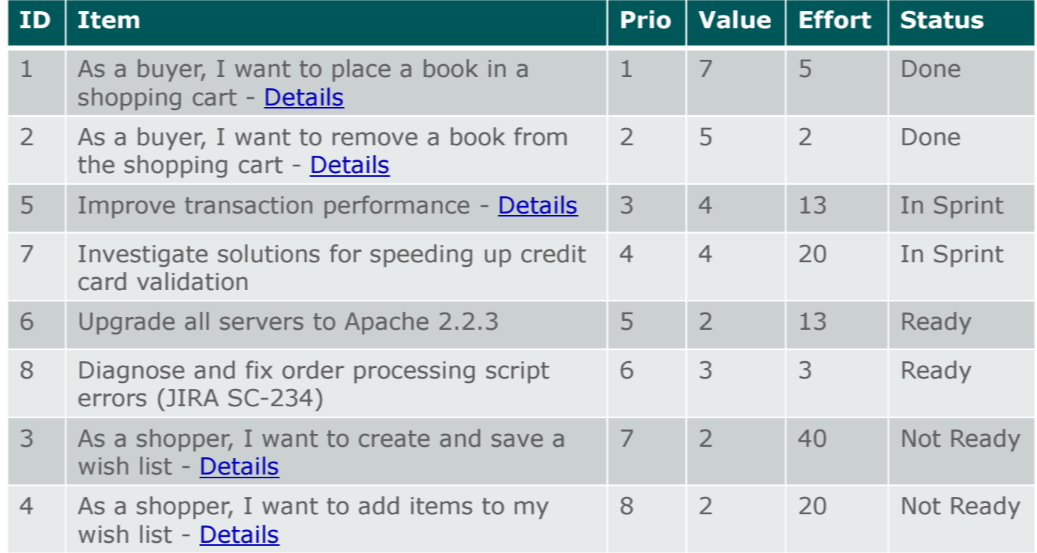
\includegraphics[width=\linewidth]{figuras/ciclo-scrum.png}
\captionof{figure}{El ciclo Scrum (cátedra).}
\end{minipage}

\textbf{Reuniones.}
\begin{itemize}
  \item \textbf{Sprint Planning}, en dos partes: \emph{el qué} (PO, SM y equipo negocian el alcance: el PO dice
  qué importa, el equipo cuánto puede comprometer) y \emph{el cómo} (el equipo descompone cada ítem en tareas
  estimadas en horas).
  \item \textbf{Backlog Refinement} (\emph{grooming}): se estiman, dividen, aclaran y repriorizan los ítems
  para el próximo sprint.
  \item \textbf{Daily Scrum}: 15 minutos, frente al tablero; cada uno responde ¿qué hice?, ¿qué voy a hacer?,
  ¿qué problemas tengo? No es un reporte al Scrum Master; los problemas se resuelven después.
  \item \textbf{Sprint Review}: se muestra \textbf{software funcionando} (no diapositivas) a PO y stakeholders;
  los cambios que surgen van al backlog.
  \item \textbf{Sprint Retrospective}: el equipo revisa su \emph{proceso} (no el producto): qué salió bien, qué
  mejorar, qué acciones tomar. Las acciones deben ser \textbf{SMART}: específicas, medibles, alcanzables,
  relevantes y acotadas en el tiempo.
\end{itemize}

\subsection{Historias de usuario, estimación y velocity}
\begin{defbox}{Historia de usuario (US) e INVEST}
``Como \textbf{[rol]}, quiero \textbf{[objetivo]}, para \textbf{[beneficio]}''. Ejemplo: ``Como comprador,
quiero agregar libros al carrito para elegir los que voy a comprar''. Una buena historia es \textbf{INVEST}:
\textbf{I}ndependiente (se puede reordenar), \textbf{N}egociable (no es un contrato cerrado),
\textbf{V}aliosa (para el usuario o quien paga), \textbf{E}stimable, \textbf{S}mall (menos de 3
semanas-persona) y \textbf{T}esteable.
\end{defbox}
Los \textbf{criterios de aceptación} hacen testeable a la historia: son condiciones verificables que suelen
combinar (a) lo que el usuario \emph{puede hacer} (``puede buscar por autor o título''), (b) las
\emph{reglas} según el caso (``si el libro ya está en el carrito, se aumenta la cantidad; si no, se agrega con
cantidad uno'') y (c) la \emph{confirmación visible} (``luego se muestra el carrito'').

\paragraph{Historia de usuario o ítem técnico.} Pregunta guía: ¿lo podría haber pedido un usuario sin
conocimientos técnicos porque necesita hacer algo nuevo? Si sí, es una historia. ``Mejorar la performance de
las transacciones'', ``investigar soluciones para validar tarjetas'', ``actualizar los servidores a Apache
2.2'' o ``corregir el script de compras'' están en infinitivo, no tienen rol y benefician al sistema: son
\textbf{ítems técnicos} del equipo.

\paragraph{Business value, story points y velocity.} El \textbf{business value} (lo aporta el PO) mide el
beneficio para el cliente. Los \textbf{story points} (los estima el equipo) miden el \emph{esfuerzo relativo}:
en vez de ``¿cuántas horas?'' se pregunta ``¿es más grande o más chica que esta otra?'', con una escala no
lineal tipo Fibonacci (1, 2, 3, 5, 8, 13, $\infty$; el infinito indica que hay que partir la historia). La
\textbf{velocity} es la cantidad de story points que el equipo completa por sprint: funciona como un
presupuesto. Al principio se estima; con varios sprints se toma el promedio real. El \textbf{burndown chart}
muestra el esfuerzo restante por día: si la línea real queda \emph{por encima} de la ideal, el sprint va
atrasado; si queda plana, el trabajo no avanza.

\begin{ejemplo}{Procedimiento de selección para el sprint (TP0)}
\small
\begin{minipage}[t]{0.47\textwidth}
\begin{tabular}{@{}clccc@{}}
\toprule
\# & Ítem & V & E & V/E\\
\midrule
2 & sacar libro del carrito & 5 & 2 & 2,50\\
1 & poner libro en carrito & 7 & 5 & 1,40\\
6 & corregir script compras & 3 & 3 & 1,00\\
8 & agregar a favoritos & 4 & 5 & 0,80\\
3 & mejorar performance & 4 & 13 & 0,31\\
4 & investigar tarjetas & 4 & 13 & 0,31\\
7 & lista de favoritos & 2 & 8 & 0,25\\
5 & upgrade Apache & 2 & 13 & 0,15\\
\bottomrule
\end{tabular}
\end{minipage}\hfill
\begin{minipage}[t]{0.5\textwidth}
Con velocity 20: (1) calcular valor/esfuerzo; (2) ordenar de mayor a menor; (3) tomar en orden acumulando
puntos sin pasarse: 2 $\to$ 2, 1 $\to$ 7, 6 $\to$ 10, 8 $\to$ 15; los siguientes (13, 13, 8, 13) no entran;
(4) verificar que ningún ítem más chico quepa en los 5 restantes. \textbf{Sprint: \#2, \#1, \#6 y \#8 (15
puntos).} El ratio \emph{orienta}: el PO puede priorizar otra cosa por dependencias, riesgos o fechas
comprometidas.
\end{minipage}
\end{ejemplo}

\paragraph{Planning Poker.} Técnica de estimación ágil (artículo recomendado por la cátedra): cada miembro del equipo que va a
construir recibe un mazo (0, 1, 2, 3, 5, 8, 13, 20, 40, 100, ``?'', $\infty$); el PO presenta la historia y
aclara dudas; todos eligen una carta \textbf{en secreto} y la muestran \textbf{a la vez}; si no coinciden, el
que puso la más alta y el que puso la más baja explican sus razones y se vuelve a votar hasta el consenso. La
revelación simultánea evita el \textbf{anclaje} (que la primera opinión, a menos que sea la del jefe, arrastre
a todos), y la discusión de los extremos saca a la luz información que solo tenía uno. Es un \emph{Delphi
ágil}. Fibonacci se usa porque la distancia entre valores crece con la incertidumbre: discutir entre 37 y 38
sería precisión falsa.

\begin{enresumen}
Ágil son valores (4) y principios (12); Scrum es un framework con 3 roles (PO, SM, equipo), artefactos
(backlogs, sprint con alcance congelado) y 5 reuniones. Las historias siguen el formato como/quiero/para,
cumplen INVEST y llevan criterios de aceptación. El PO da el valor, el equipo los story points; la velocity
limita lo que entra en el sprint y el ratio valor/esfuerzo orienta el orden.
\end{enresumen}

% =====================================================================
\section[Proyectos: definición, parámetros, clasificación y etapas]{Proyectos: definición, parámetros, clasificación y etapas \hfill {\normalsize [TP1 §1--7]}}
% =====================================================================
\subsection{Qué es un proyecto y qué es administrarlo}
\begin{defbox}{Proyecto}
Una \textbf{secuencia de actividades} con un \textbf{propósito}, que debe completarse en un \textbf{tiempo}
determinado, dentro de un \textbf{presupuesto} y de acuerdo a una \textbf{especificación}. Dicho corto:
cualquier actividad que dé como resultado un producto o entregable.
\end{defbox}
Cada palabra tiene consecuencias: las actividades son \textbf{únicas} (nunca se hicieron igual; eso separa un
proyecto de una operación rutinaria), \textbf{complejas}, \textbf{conectadas} (hay dependencias), con un
\textbf{propósito simple} y bajo \textbf{tiempo, presupuesto y especificación} (que puede variar). Todo
proyecto \textbf{comienza con el enunciado de un problema}. Se evalúa desde cuatro preguntas: ¿resuelve el
problema del usuario?, ¿el usuario está satisfecho con el \emph{proceso}?, ¿lo está la gerencia?, ¿lo está el
equipo? El ambiente actual es de \emph{alta velocidad, alto cambio, bajos costos, alta complejidad y alta
incertidumbre}, y exige flexibilidad, comprensión del negocio y hacerse cargo del proyecto.

\textbf{Administración de proyectos} (PMI): aplicar conocimientos, habilidades, herramientas y técnicas a las
actividades de un proyecto para satisfacer sus requerimientos. En software, combinar administración e
ingeniería para entregar con \textbf{mínimo costo}, \textbf{mínimo tiempo} y \textbf{buena calidad}. Los datos
que da la cátedra: menos de un tercio de los proyectos termina en tiempo y presupuesto, pero con una cultura de
gestión fuerte el 71\% cumple sus objetivos. Desafíos: innovación, complejidad, requerimientos ambiguos, falta
de competencias, herramientas inmaduras, regulaciones, plazos, proveedores, retener personal, equipos
distribuidos y multiculturales.

\subsection{Parámetros, triángulo de alcance y corrimientos}
\begin{minipage}[t]{0.6\textwidth}
Todo proyecto se mueve dentro de \textbf{cinco parámetros}, que también son sus restricciones:
\textbf{ámbito} (alcance: qué se hace y qué no), \textbf{calidad}, \textbf{costo}, \textbf{tiempo} y
\textbf{recursos} (personas, equipos, licencias). No son independientes: el \textbf{triángulo de alcance}
tiene vértices \emph{tiempo}, \emph{costo} y \emph{alcance y calidad}, y mover uno obliga a mover otro. Si el
cliente pide más funcionalidad con la misma fecha, sube el costo (más recursos) o baja la calidad. Sirve para
\textbf{escalar problemas} (un atraso no se arregla ``por arte de magia'') y como \textbf{base para definir el
impacto de un cambio}. El proyecto es un sistema dinámico que el LP mantiene en equilibrio.
\end{minipage}\hfill
\begin{minipage}[t]{0.36\textwidth}\vspace{0pt}\centering
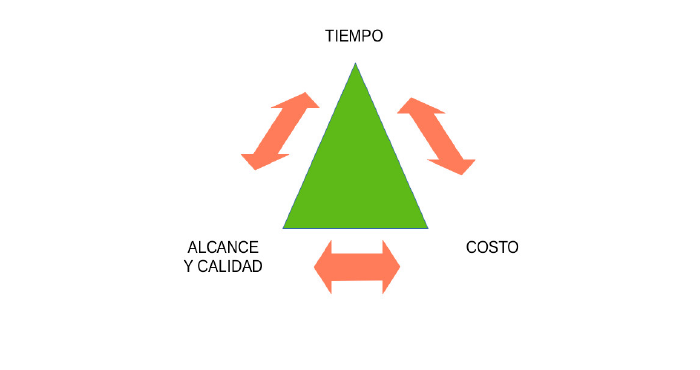
\includegraphics[width=0.85\linewidth]{figuras/triangulo.png}
\captionof{figure}{Triángulo de alcance (cátedra).}
\end{minipage}

\textbf{Quién controla qué}: el \textbf{líder de proyecto} controla la utilización de los recursos y el
cronograma; el \textbf{gerente}, los niveles de recursos y los costos; el \textbf{cliente}, el alcance, la
calidad y las fechas de entrega. Si el cliente pide un cambio, decide él, pero el LP traduce el impacto y el
gerente decide si pone recursos.

\textbf{Corrimientos} (desvíos progresivos y silenciosos de un parámetro):
\begin{itemize}
  \item \textbf{De alcance} (\emph{scope creep}): todo cambio que no estaba en el plan. El LP debe acomodar el
  proyecto (con el proceso de cambios), no ignorarlo.
  \item \textbf{De esperanza} (\emph{hope creep}): reportar ``sin demoras'' esperando recuperar antes del próximo
  informe. Se combate verificando los informes, por ejemplo con \textbf{controles aleatorios}.
  \item \textbf{De esfuerzo} (\emph{effort creep}): se trabaja y se reporta avance, pero la tarea nunca termina.
  \item \textbf{De rasgos} (\emph{feature creep}): el equipo agrega características que nadie pidió; cada una
  necesita pruebas, datos, documentación y capacitación, y consume tiempo y costo sin autorización.
\end{itemize}

\subsection{Éxito y fracaso}
Un proyecto puede fracasar \textbf{al comienzo} (no se planificó: avanza rápido hasta el 90\% y se queda ahí),
\textbf{durante el desarrollo} (análisis y diseño mal documentados, responsabilidades confusas, falta de
planificación de recursos, codificación prematura, sin revisiones gerenciales ni \emph{walk-throughs}, sin
estándares, deserciones, ``fuerza bruta'' de horas extra) o \textbf{al final} (pocas pruebas, mala
performance, mantenimiento caro, cancelación por fondos, contexto, gente clave o desastre técnico). Para la
cátedra, planificar es saber \textbf{a dónde} se va, \textbf{cómo} se llega y \textbf{cómo se prueba} que se
llegó. Los proyectos \textbf{exitosos} tienen un comienzo claro con plan detallado, criterios de medición
aceptables, monitoreo cercano, documentación clara y revisiones frecuentes, procedimientos para detectar
problemas y un costo razonablemente cercano al estimado.

\subsection{Clasificación de proyectos (A--D)}
Cada proyecto es único, pero no se puede inventar un proceso para cada uno: se clasifican para aplicar
\textbf{políticas por grupo}. Criterios: riesgo, valor para el negocio, duración, complejidad, tecnologías
(conocidas a nunca usadas), departamentos afectados y costo.
\begin{center}\small
\begin{tabular}{@{}c l l l l l l@{}}
\toprule
\textbf{Tipo} & \textbf{Duración} & \textbf{Riesgo} & \textbf{Complejidad} & \textbf{Tecnología} & \textbf{Complicaciones} & \textbf{Planificar}\\
\midrule
A & $>18$ meses & alto & alta & de avanzada & seguras & 5 días o más\\
B & 9--18 meses & medio & media & actual & alta probabilidad & 3--4 días\\
C & 3--9 meses & bajo & baja & buena & alguna probabilidad & hasta 2 días\\
D & $<3$ meses & muy bajo & muy baja & práctica & ninguna & menos de 1 día\\
\bottomrule
\end{tabular}
\end{center}
\textbf{A}: alto valor y alta complejidad, merecen todos los recursos (una tecnología nueva en un producto
clave). \textbf{B}: más cortos pero significativos y tecnológicamente desafiantes. \textbf{C}: los más
frecuentes; unas 5 personas hasta 6 meses, con recursos no dedicados. \textbf{D}: apenas son proyectos (cambios
menores en un proceso). No todos los procesos son obligatorios: \textbf{el POS es requerido en los cuatro
tipos}, igual que la aprobación del pedido, la propuesta y su aprobación, el cronograma, el reporte de estado,
la aprobación de entregables y la auditoría post-implementación. Las condiciones de satisfacción, la sesión de
planificación, el kick-off, las reuniones de equipo y las notas del proyecto son \emph{opcionales} en C y D.

\subsection{Etapas, hitos y ciclos de vida}
\label{sec:etapas}
Para controlar algo hay que descomponerlo: en partes del producto, en trabajo de personas y en \textbf{fases de
tiempo}. Cada fase produce uno o más \textbf{hitos}: eventos que prueban claramente que una etapa concluyó
satisfactoriamente (entrega del documento de requerimientos, de la especificación, del diseño, del código, el
deploy). Los cinco procesos típicos son:
\begin{itemize}
  \item \textbf{Concepción} (\emph{scoping}): define \textbf{qué} se hará, incluidos los criterios de éxito:
  reclutar al LP, obtener y documentar las reales necesidades, negociar cómo se cubrirán, escribir el POS y
  ganar la aprobación para planificar.
  \item \textbf{Planificación}: define \textbf{cómo}: definir el trabajo, estimar tiempo, recursos y costo,
  secuenciar, cronograma inicial, \textbf{plan de contención de riesgos}, documentar y ganar la aprobación para
  lanzar.
  \item \textbf{Lanzamiento}: reclutar el equipo, emitir la descripción del proyecto, reglas del equipo,
  \textbf{proceso de cambio de alcance}, comunicaciones, terminar el cronograma, paquetes de trabajo.
  \item \textbf{Monitoreo y control}: medir la performance, reportes de estado, monitorear riesgos, procesar
  pedidos de cambio, descubrir y resolver problemas.
  \item \textbf{Cierre}: aprobación del cliente, instalación de entregables, reporte final, auditoría
  post-implementación.
\end{itemize}
Las combinaciones dan los \textbf{ciclos de vida}: \emph{concepción--planificación--lanzamiento} (una o dos
personas: sirve como lista de tareas); \emph{más control} (lanzar es solo el 50\%: el control anticipa
problemas); \emph{las cinco etapas} (el LP aprende de la experiencia del proyecto terminado).

\subsection{Atributos críticos}
\begin{defbox}{Atributo crítico}
Una calidad o un recurso que puede hacer \textbf{colapsar el sistema} si supera ciertos límites (su
\textbf{peor caso aceptable}). Se especifica con niveles medibles, no con una frase vaga.
\end{defbox}
\begin{ejemplo}{Capacidad de trabajo (cátedra)}
Debe alcanzar para el trabajo diario normal. \emph{Peor caso}: 4 s promedio por transacción. \emph{Nivel
planificado}: menos de 1 s (0,2 s si hay más de 100.000 transacciones diarias). \emph{Mejor caso}: 0,1 s. En el
caso real se ``presumió'' que habría capacidad suficiente, y como nunca se escribió como requerimiento, nadie la
verificó.
\end{ejemplo}
\textbf{Principios de administración}: especificar claramente todos los atributos críticos; satisfacerlos
\emph{simultáneamente}; en términos testeables y medibles, identificando el peor caso; \textbf{nunca} entregar
sistemas grandes y complejos de una sola vez (\emph{big-bang}); no creer ciegamente en ningún método; ``si no se
sabe lo que se está haciendo, no hacerlo en gran escala''.

\begin{enresumen}
Proyecto: actividades únicas, complejas y conectadas, con propósito, tiempo, presupuesto y especificación.
Cinco parámetros en tensión (triángulo tiempo--costo--alcance/calidad); el LP controla recursos y cronograma,
el gerente niveles de recursos y costos, el cliente alcance, calidad y fechas. Cuatro corrimientos. Tipos A a
D; el POS siempre es obligatorio. Cinco etapas con hitos. Atributos críticos con peor caso medible.
\end{enresumen}

% =====================================================================
\section[Concepción: COS, POS y aprobación]{Concepción: COS, POS y aprobación \hfill {\normalsize [TP1 §8, TP2 §1--3 y §6]}}
% =====================================================================
\subsection{La falla de comunicación cliente--proveedor}
La causa más común de fracaso no es técnica sino \textbf{comunicacional}: se construye algo distinto de lo que
el cliente necesitaba. Los clientes esperan más de lo que los proveedores están preparados para entregar, y
hay \textbf{dos supuestos encadenados que nadie verifica}: que el LP entendió lo que pidió el
\emph{requiriente} (el cliente), y que lo que el cliente pidió es lo que realmente necesita. Por eso el LP
pregunta \textbf{por qué} lo quiere, no solo qué quiere. \textbf{Regla de oro}: nunca comenzar un proyecto sin
estar seguro de que la solución propuesta es lo que realmente satisface al cliente. Las herramientas de la
concepción (se eligen según el proyecto) son: COS, POS, reuniones de definición, especificación de
requerimientos, diagramación de procesos de negocio, prototipos, validación de casos de uso, administración de
la provisión, outsourcing y aprobación para la planificación.

\subsection{Condiciones de Satisfacción (COS)}
\begin{defbox}{COS}
Una \textbf{conversación estructurada} (un proceso, no un documento) entre el requiriente y el probable LP para
llegar a un entendimiento compartido de qué se va a hacer. Su producto tangible es el POS.
\end{defbox}
Tiene \textbf{cuatro etapas cíclicas}:
\begin{enumerate}
  \item \textbf{Requerimiento}: el cliente pide, en el lenguaje de su negocio.
  \item \textbf{Clarificación}: el proveedor explica con sus palabras lo que entendió, \emph{en el lenguaje del
  requiriente}.
  \item \textbf{Respuesta}: el proveedor dice qué es capaz de proveer (lo pedido, una parte o una alternativa).
  \item \textbf{Acuerdo}: el requiriente explica con sus palabras lo que entendió que se le ofrece.
\end{enumerate}
Obligar a ambos a \emph{parafrasear}, en lugar de asentir, hace visibles los malentendidos cuando corregirlos
cuesta una charla. Lo normal es que no haya acuerdo en la primera vuelta. Datos operativos: el entregable es el
POS de \textbf{una página}, firmado por ambas partes; la concepción termina cuando lo aprueba un \textbf{gerente
senior}; el COS sirve mejor en proyectos pequeños y medianos; es \textbf{dinámico}: se especifica qué productos
demostrarán que se cumplió (criterios de éxito) y se revisa durante el monitoreo.

\subsection{El POS (Project Overview Statement)}
\begin{defbox}{POS --- Enunciado General del Proyecto}
Documento breve de la concepción que dice \textbf{qué} se va a hacer, \textbf{por qué} y \textbf{qué valor
comercial} tendrá. Esquema de las diapositivas: nombre y número del proyecto, líderes, \textbf{problema/oportunidad},
\textbf{metas}, \textbf{objetivos}, \textbf{criterios de éxito}, \textbf{suposiciones, riesgos y
obstáculos}, preparado por/fecha, aprobado por/fecha.
\end{defbox}
Funciones organizacionales: base para \textbf{aprobar y autorizar recursos}; insumo para \textbf{priorizar la
cartera} de proyectos (casi siempre hay más ideas que recursos); \textbf{referencia para la planificación};
\textbf{solicitud} formal de la iniciativa. Cada campo responde una pregunta distinta:
\begin{center}\small
\begin{tabularx}{\textwidth}{@{}l X X@{}}
\toprule
\textbf{Campo} & \textbf{Qué debe decir} & \textbf{Ejemplo}\\
\midrule
Problema / oportunidad & la situación actual insatisfactoria o la ventaja no aprovechada, \emph{sin proponer la
solución ni comprometer métricas} & ``El instituto gestiona los alumnos con planillas Excel; esto produce una
distribución inadecuada de la información y servicios ineficientes.''\\
Meta & la finalidad del proyecto; cualitativa, corta, sin fechas necesariamente; verbo como facilitar, lograr,
mejorar; debe hacer que la gerencia quiera seguir leyendo & ``Facilitar el acceso de los usuarios a sus datos
personales para que puedan modificarlos.''\\
Objetivos & el desglose de la meta: \textbf{medibles y con plazo}; conjunto \textbf{necesario} (todos aportan)
y \textbf{suficiente} (entre todos alcanzan) & ``El 80\% de los usuarios accede a sus datos a menos de una
semana de la puesta en producción.''\\
Criterios de éxito & métricas cuantitativas que prueban que el proyecto cumplió lo prometido; pueden mirar al
equipo o la organización & ``Satisfacción de los usuarios de al menos 4 sobre 5.''\\
Suposiciones, riesgos y obstáculos & lo que se da por sentado o podría hacer fracasar o demorar el proyecto
(conecta el POS con el análisis de riesgos) & ``Se supone que la prepaga acepta renegociar; los datos de salud
son sensibles.''\\
\bottomrule
\end{tabularx}
\end{center}
\textbf{Objetivos bien escritos}: las cinco características (específicos, medibles, \emph{asignables} a un
responsable, realistas y limitados en el tiempo) y los cuatro componentes (una \emph{salida}, un \emph{marco de
tiempo}, una \emph{medida} y una \emph{acción}). Si en esta etapa se dan estimaciones, hay que aclarar que son
\emph{preliminares}.

\begin{defbox}{FCE (Factores Críticos de Éxito) vs.\ criterios de éxito}
Un \textbf{FCE} responde ``¿qué debería sucedernos a nosotros y al cliente para decir que el proyecto fue un
éxito?''. Son pocos, decisivos, medibles y en términos de negocio; sirven para ``vender'' el proyecto y que la
gerencia autorice recursos. Los \textbf{criterios de éxito} son su operacionalización: las métricas que
verifican que el FCE se cumplió. Ej.: FCE ``que el área de ventas adopte el sistema y abandone el proceso
manual''; criterio ``el 90\% de las órdenes del trimestre se carga por el sistema''.
\end{defbox}

\subsection{Aprobación para la planificación}
Terminado el POS, se envía con sus adjuntos a los gerentes senior. No es un trámite: evalúan si el proyecto
tiene valor y está bien definido. \textbf{Aprobar el POS es asignar recursos para planificar en detalle}; la
aprobación del proyecto para ejecutarlo viene después, con el plan. Puede haber varias iteraciones. Cumple una
función para tres audiencias: a la \emph{alta gerencia} le justifica dedicar recursos; al \emph{cliente} le
muestra que el proyecto está bien definido; al \emph{equipo} le asegura que gerencia y cliente están
alineados. Participan el LP, los gerentes de los recursos (de usuarios), los gerentes de los procesos que
intercambian información con el sistema, el cliente y la alta gerencia. Los gerentes suelen preguntar por la
importancia del problema, la relación con los FCE, si la meta responde al problema, si los objetivos
representan la meta, si el valor de negocio justifica el gasto y si se pueden mitigar los riesgos.
\textbf{Resultados posibles}: \textbf{aprobado}, \textbf{rechazado}, \textbf{reformulación} (se reenvía),
\textbf{postergado} o \textbf{derivado a un portafolio}.

\begin{enresumen}
El COS es una conversación en cuatro etapas (requerimiento, clarificación, respuesta, acuerdo) cuyo resultado
es el POS: una página, firmada, con problema (sin solución), meta (cualitativa), objetivos (medibles, con
plazo, necesarios y suficientes), criterios de éxito y riesgos. Los FCE venden el proyecto; los criterios los
miden. La aprobación del POS habilita a planificar, no a ejecutar.
\end{enresumen}

% =====================================================================
\section[Requerimientos y soluciones]{Requerimientos y soluciones \hfill {\normalsize [TP2: apunte de Requerimientos y §4]}}
\label{sec:req}
% =====================================================================
\subsection{Requerimientos: definición, proceso y tipos}
\begin{defbox}{Requerimiento}
Equivalentemente: (1) una función que el sistema debe realizar; (2) una característica deseada del sistema;
(3) un enunciado sobre el sistema que los \emph{stakeholders} acuerdan que debe satisfacerse para que el
problema del cliente quede adecuadamente resuelto.
\end{defbox}
La tercera definición es la importante para la gestión: un requerimiento nace de un \emph{acuerdo} y existe
para \emph{resolver un problema}. Un \textbf{stakeholder} (interesado) es cualquier persona u organización cuyos
intereses se ven afectados por el proyecto (cliente, usuarios, gerencia, equipo, soporte, reguladores).

\textbf{El proceso de requerimientos} tiene cinco actividades, \textbf{no lineales} (se realimentan):
\textbf{elicitación} (descubrir los requerimientos con los stakeholders), \textbf{especificación}
(documentarlos de forma clara y sin ambigüedad; el SRS), \textbf{modelamiento y análisis} (representarlos con
modelos y detectar faltantes, contradicciones o imposibles), \textbf{validación} (confirmar con los
stakeholders que son los requerimientos \emph{correctos}) y \textbf{administración} (gestionar cambios y
trazabilidad durante todo el proyecto).

\begin{center}\small
\begin{tabularx}{\textwidth}{@{}l X X@{}}
\toprule
 & \textbf{Requerimiento funcional} & \textbf{Requerimiento no funcional}\\
\midrule
Definición & Describe la interacción entre el sistema y su entorno: cómo se comporta ante un estímulo. &
Describe restricciones que \textbf{limitan la selección de soluciones}: con qué calidad o bajo qué límites.\\
Cumplimiento & \textbf{Presente o ausente} en un plan o sistema (binario). & Tiene una \textbf{escala de
demanda} y admite negociación según las prioridades.\\
Se gestiona como & lista de ítems (está o no está en el alcance). & atributo con escala, test y niveles.\\
Ejemplo & ``El sistema permite registrar un nuevo usuario.'' & ``El registro se completa en menos de 2 s.''\\
\bottomrule
\end{tabularx}
\end{center}
\textbf{Tipos} usados para organizar el documento: funcional, de interfaz (con otros sistemas o dispositivos),
de datos, de ingeniería humana (usabilidad), operacionales (disponibilidad, backups, soporte), restricciones
de diseño (``debe usar tal lenguaje''), de seguridad, etc.

\textbf{Cualidades de una buena especificación}: \textbf{correcta} (refleja una necesidad real),
\textbf{consistente} (sin contradicciones), \textbf{factible}, \textbf{verificable} (hay forma objetiva de
comprobarla), \textbf{completa} y \textbf{trazable} (hacia su origen y hacia el diseño, código y pruebas).
\textbf{Estándares} que listan las diapositivas: Guía IEEE P1233/D3, Guía IEEE Std.\ 1233, IEEE Std.\ 830-1998,
ISO/IEC 12119-1994 e IEEE Std.\ 1362-1998 (ConOps).

\subsection{Funcionales: separar función, calidad y solución}
Lo esencial es identificar las \textbf{funciones} del sistema (algo que el sistema hace). Suelen registrarse
como una lista que completan los usuarios con ayuda del analista. Dos errores clásicos:
\begin{itemize}
  \item \textbf{Mezclar función y calidad}: ``redactar un manual de usuario \emph{legible}''. ``Redactar un
  manual'' es funcional (está o no está); ``legible'' es un atributo (escala). Hay que separarlos para poder
  verificar cada parte.
  \item \textbf{Soluciones disfrazadas de requerimientos}: lo que el usuario enuncia en la elicitación suele ser
  su forma de decir lo que desea, no la mejor solución. Si se registra como requerimiento, se cierra la puerta a
  alternativas. Técnica: preguntar \textbf{¿por qué?} o \textbf{¿para qué?} hasta llegar a la necesidad real.
  ``El usuario requiere construir estándares'' $\to$ ¿para qué? $\to$ para facilitar el mantenimiento y
  posibilitar la rotación de personal.
\end{itemize}
\begin{ejemplo}{El ejercicio del apunte}
``Nosotros, la organización XX, queremos escribir un manual de desarrollo de sistemas para mejorar
sustancialmente la productividad del personal.'' \textbf{No funcional}: mejorar sustancialmente la
productividad (se mide en una escala; es el objetivo real). \textbf{Funcional}: escribir el manual (está o no
está). \textbf{Solución}: el manual, elegido de antemano; hay que cuestionarlo, porque quizás una capacitación o
mejores herramientas mejoran más la productividad.
\end{ejemplo}

\begin{center}\small
\begin{tabularx}{\textwidth}{@{}l X@{}}
\toprule
\multicolumn{2}{@{}l}{\textbf{Ficha de un requerimiento funcional (ejemplo de las slides)}}\\
\midrule
req.\ id / categoría & F44 / Funcional\\
descripción & Aplicantes a beneficios, empleados y autoridades deben poder registrarse; se crea una cuenta para
autenticación y personalización. Los empleados los crea el administrador; los aplicantes se registran solos en
el portal.\\
términos & Cuenta, Aplicante, Autenticación, Registración, Usuario (glosario para que todos entiendan lo mismo).\\
justificación / prioridad & Esencial para autenticar y personalizar / Alta.\\
dependencias / documentos & F43 / ---\\
factibilidad & Existen soluciones maduras (servicios de directorio).\\
verificación & Al registrar un aplicante sin cuenta, se crea una cuenta en el sistema.\\
\bottomrule
\end{tabularx}
\end{center}
Cada campo fuerza una cualidad: id y dependencias $\to$ trazabilidad; justificación $\to$ correcta;
factibilidad $\to$ factible; verificación $\to$ verificable.

\subsection{No funcionales: atributos, escala, test y niveles}
\begin{defbox}{Atributo}
Un \textbf{concepto de calidad o de recurso} que describe el sistema \textbf{cuantitativamente}; representa
restricciones y se define para cada proyecto. Los atributos de calidad constituyen los requerimientos no
funcionales.
\end{defbox}
\begin{itemize}
  \item La \textbf{especificación de atributos} es una lista estructurada, con historial de cambios; los
  atributos críticos se controlan durante todo el ciclo de vida. Todos deberían volverse medibles: la gente
  falla al definir escalas porque culturalmente no se exige.
  \item Se organizan en \textbf{jerarquías}: ``mejor calidad y organización más productiva'' $\to$ satisfacción
  de clientes, productividad de sistemas, adaptabilidad de los empleados. Se descompone hasta el nivel que
  permita controlar. Si son más de 7 a 10, se agrupan bajo un nombre corto (``Performance del sistema'': carga
  semanal, disponibilidad, tiempo de respuesta).
  \item Conviene identificar primero los de \textbf{bajo nivel} (concretos, visibles) y subir preguntando
  \emph{por qué}: el de alto nivel muestra otras soluciones (el usuario pide ``confiabilidad'' y en realidad
  quiere \emph{disponibilidad}, que también depende de mantenibilidad e integridad).
  \item Se especifican \textbf{al principio}, antes de cualquier solución, en lenguaje que entiendan todos (la
  prueba es que la gerencia usuaria firme), y \textbf{no se congelan}. Las soluciones se juzgan contra
  \emph{todos} los atributos juntos.
  \item Si cuesta definir una medida, el atributo es de alto nivel: ``amigable'' $\to$ aprendizaje (horas para
  aprender, planificado 5) y productividad (tareas por hora, planificado 20).
\end{itemize}
\begin{center}\small
\begin{tabularx}{\textwidth}{@{}l X l@{}}
\toprule
\textbf{Campo} & \textbf{Significado} & \textbf{Ejemplo: tiempo de actualización}\\
\midrule
Escala & unidad de medida, \emph{qué} se mide (voltios) & ms desde el evento hasta la BD actualizada\\
Test & procedimiento, \emph{cómo} se mide (voltímetro); mejor si ya está en uso & un día aleatorio, mínimo 10 casos, ideal 50\\
Peor caso & peor nivel aceptable bajo cualquier circunstancia: por debajo hay \textbf{fracaso}; base de un contrato & 180.000 ms\\
Nivel planificado & lo que el proyecto \textbf{se compromete} a lograr (éxito formal); realista pero ambicioso, no la perfección & 100 ms\\
Mejor caso & lo mejor alcanzado en cualquier circunstancia: \textbf{solo informativo}, ``límite de la ingeniería'' & 1 ms\\
Nivel actual & valor en un sistema existente (citar la fuente); planificado $-$ actual $=$ mejora prometida & sin medida\\
\bottomrule
\end{tabularx}
\end{center}
De peor a mejor: peor caso $\to$ (nivel actual) $\to$ nivel planificado $\to$ mejor caso. Para fijar el peor
caso: imaginar un nivel inaceptable e irlo mejorando hasta que algún usuario lo acepte en alguna circunstancia.

\subsection{Soluciones}
\label{sec:soluciones}
El ejemplo de la \textbf{hamaca} (lo que pidió el cliente, lo que entendió el vendedor, lo que diseñó el
equipo\ldots) muestra que la función (``una hamaca colgada de un árbol'') era clara; lo que falló fue la
especificación de \textbf{atributos}: la calidad y los recursos de cada etapa.
\begin{defbox}{Solución}
Un \textbf{conjunto de ideas cuya implementación impacta positivamente en al menos una parte del problema}. Una
idea sin efectos positivos en los requerimientos no es una solución. Es válida \emph{en la medida en que mejor
sirva a los requerimientos actuales}: si estos cambian, puede dejar de serlo.
\end{defbox}
\begin{itemize}
  \item Hay que tener soluciones suficientes para \textbf{todos los objetivos del POS}. Se empieza por las
  funciones (más visibles). Cadena: \emph{las funciones determinan los atributos y los atributos determinan las
  soluciones}.
  \item Para evaluar una solución hace falta: requerimientos especificados, sus contribuciones positivas, sus
  efectos colaterales negativos y su consumo de recursos frente al presupuesto.
  \item Requerimiento funcional $=$ un estado futuro verdadero o falso; no funcional $=$ escala; solución $=$ una
  idea que impacta en ellos. \textbf{Que una solución no se transforme en un requerimiento.}
  \item \textbf{Flexibilidad}: una solución puede especificarse como \emph{requerimiento funcional} (solo si es
  más prioritaria que el atributo que perjudica), como solución \emph{para un rango} de un atributo (para evitar
  extremos) o como \textbf{non-sancta} (sujeta a cambios: el caso por defecto).
  \item Los \textbf{gerentes} enuncian sus problemas en términos de objetivos; los \textbf{problem solvers}
  encuentran las soluciones. Son procesos separados.
  \item \textbf{Mapeo}: varias soluciones pueden impactar en un atributo, una solución en varios, y algún
  atributo puede no tener solución (hay que revisar si el objetivo es alcanzable).
  \item \textbf{Estimación del impacto}: cuánto contribuye cada solución a cada atributo, expresado como
  estimación o \emph{rango} (incertidumbre honesta), en una \textbf{tabla de estimación de impacto}. Beneficios:
  permite discutir con el decisor, entrena a estimar, motiva a cumplir, habilita la discusión profesional y
  aclara objetivos mal expresados.
  \item \textbf{Comparación}: técnica tabular que asegura consistencia y comunicación. Se \textbf{suman
  algebraicamente} los impactos: en calidad, más es mejor; en recursos, menos es mejor.
  \[ \text{Razón de impactos} = \frac{\sum \text{impactos de calidad}}{\sum \text{impactos de recursos}} \quad (\text{mayor es mejor}) \]
  \item \textbf{Proceso de 7 pasos}: (1) un atributo por vez, lluvia de ideas; (2) estimar efectos colaterales;
  (3) \textbf{eliminar las que producen el peor caso} en algún atributo; (4) repetir; (5) si se cubren todos los
  niveles planificados, ir al 7; (6) si no, buscar más experiencia o negociar los niveles; (7) testear las
  hipótesis (inspección de Fagan, entregas parciales y medición).
  \item \textbf{Especificar soluciones}: resumidas, precisas, cada idea nueva en su propio enunciado, con una
  \textbf{etiqueta} única (numérica o mnemotécnica, que no envejece; jerárquica; temporal para versiones), útil
  para tablas y gestión de configuración.
\end{itemize}

\begin{ejemplo}{Comparación de soluciones (TP2, ejercicio 5)}
\small
\begin{minipage}[t]{0.38\textwidth}\centering
\begin{tabular}{@{}lccc@{}}
\toprule
 & S1 & S2 & S3\\
\midrule
A & 20 & 30 & 10\\
B & 80 & 10 & 50\\
C & 5 & 20 & 50\\
D & 15 & 20 & 50\\
\midrule
Suma & 120 & 80 & \textbf{160}\\
Costo & 40\% & 40\% & 70\%\\
Razón & \textbf{3,00} & 2,00 & 2,29\\
\bottomrule
\end{tabular}
\end{minipage}\hfill
\begin{minipage}[t]{0.6\textwidth}
Cada celda es el \% del nivel planificado del atributo que aporta la solución.
(a) Por impacto se elige \textbf{S3} (160), que además es la más pareja (S1 deja C en 5\%, casi el peor caso).
(b) Atributo \textbf{determinante}: se excluye uno por vez y se recalcula; sin C, S1 suma 115 y S3 110: la
preferencia cambia, así que \textbf{C} es determinante.
(c) Con costos, la razón favorece a \textbf{S1} (3,00).
(d) El líder de S2 puede \emph{reconsiderar la implementación} (siempre válido: bajar costo o mejorar B) o la
\emph{relevancia de los atributos} (solo si se acuerda con quien fija los objetivos, no para hacer ganar a S2).
\end{minipage}
\end{ejemplo}

\textbf{Inspección de Fagan}: revisión formal de \emph{documentación} por \textbf{colegas de todos los niveles
salvo el gerente} (para que la crítica sea honesta), en \textbf{puntos prefijados}, buscando \textbf{todo tipo
de defecto}, con pasos predefinidos (preparación individual, reunión, reconstrucción de errores), reuniones de
\textbf{hasta 2 horas}, un \textbf{moderador entrenado}, \textbf{roles} asignados y \textbf{checklists} de
preguntas.

\begin{enresumen}
Funcional $=$ presente/ausente; no funcional $=$ escala negociable. Se separa función de calidad y se pregunta
``¿por qué?'' ante soluciones disfrazadas. Un atributo se especifica con escala, test, peor caso, nivel
planificado, mejor caso y nivel actual. Las soluciones se comparan sumando impactos y con la razón calidad/
recursos; se eliminan las que producen el peor caso.
\end{enresumen}

% =====================================================================
\section[Gestión de riesgos]{Gestión de riesgos \hfill {\normalsize [TP1 §9, TP2 §5]}}
\label{sec:riesgos}
% =====================================================================
\subsection{Qué es un riesgo y cómo se clasifica}
\begin{defbox}{Riesgo y gestión del riesgo}
Un riesgo es un \textbf{problema potencial}: puede ocurrir o no. Implica \textbf{incertidumbre} (si fuera
seguro, sería una restricción: no existe un riesgo 100\% probable) y \textbf{pérdida} (consecuencias, impacto).
El análisis y la gestión del riesgo son pasos para comprender y gestionar la incertidumbre: (1)
\textbf{identificar}, (2) evaluar la \textbf{probabilidad}, (3) estimar el \textbf{impacto}, (4) elaborar el
\textbf{plan RSGR}. Los planes de contingencia deben ser \emph{realistas}.
\end{defbox}
\textbf{Estrategia reactiva} (``escuela Indiana Jones'': ``no te preocupes, pensaré en algo''; a lo sumo
supervisa) vs.\ \textbf{proactiva} (la recomendada: empieza \emph{antes} del trabajo técnico, identifica, valora
y prioriza, y establece un plan). ``Si no atacamos activamente a los riesgos, ellos nos atacarán.'' Principios:
el profesional \emph{comparte} el conocimiento de los riesgos con colegas y clientes; la prevención es más
efectiva en costo que la detección; al indicar desvíos se dan causas y acciones; el riesgo nunca se oculta a los
\emph{decision-makers}; si no se busca información de riesgo, se buscan problemas.

\begin{center}\small
\begin{tabularx}{\textwidth}{@{}l X@{}}
\toprule
\textbf{Clasificación} & \textbf{Categorías}\\
\midrule
Pressman & \textbf{Del proyecto}: amenazan el plan (presupuesto, calendario, personal, cliente, requisitos,
tamaño, recursos). \textbf{Técnicos}: el problema es más difícil de lo que se creía (diseño, implementación,
interfaces, mantenimiento, tecnología incierta). \textbf{Del negocio}: amenazan la viabilidad; subtipos de
\emph{mercado} (nadie lo quiere), \emph{estratégico} (no encaja en la estrategia), de \emph{ventas} (no se
sabe venderlo), de \emph{dirección} (se pierde el apoyo gerencial), de \emph{presupuesto} (se pierden fondos o
personal).\\
Genérico / específico & Genéricos: amenazan a todo proyecto. Específicos: propios de este proyecto; solo los
identifica gente con experiencia en su tecnología, personal y entorno.\\
Charette & \textbf{Conocidos} (del análisis del proyecto, su entorno y su plan), \textbf{predecibles} (se
extrapolan de otros proyectos), \textbf{impredecibles} (muy difíciles de anticipar).\\
Componentes (qué amenazan) & Riesgo de \textbf{rendimiento} (que el producto no cumpla), de \textbf{costo}
(presupuesto), de \textbf{soporte} (poder corregirlo y adaptarlo) y de \textbf{planificación temporal}
(entregar a tiempo). El impacto de cada controlador: despreciable, marginal, crítico, catastrófico.\\
\bottomrule
\end{tabularx}
\end{center}

\subsection{Herramientas para identificarlos}
La \textbf{identificación} es un intento \emph{sistemático} de especificar las amenazas al plan. Dos
herramientas, que se combinan (las categorías de Pressman son las carpetas; los conductores de Wysocki y los
riesgos específicos del enunciado, lo que va adentro):
\begin{center}\small
\begin{tabularx}{\textwidth}{@{}l X@{}}
\toprule
\multicolumn{2}{@{}l}{\textbf{Lista de comprobación de elementos de riesgo (Pressman)}}\\
\midrule
Tamaño del producto & tamaño en LDC o PF y confianza en esa estimación; BD y transacciones; desvío respecto de
proyectos similares; cantidad de usuarios; cambios previstos; cantidad de software reutilizado.\\
Impacto en el negocio & efecto en los ingresos; viabilidad según expertos; razonabilidad de la fecha; clientes
con necesidades inconsistentes; interoperabilidad; sofisticación del usuario; documentación; regulaciones;
costo del retraso y de un producto defectuoso.\\
Características del cliente & ¿trabajamos antes con él?, ¿sabe lo que quiere y lo escribió?, ¿acepta
reuniones?, ¿se comunica?, ¿participa de revisiones?, ¿deja trabajar?, ¿entiende el proceso de software?\\
Definición del proceso & ¿la gerencia apoya un proceso estándar?, ¿hay proceso escrito?, ¿revisiones
formales y documentadas?, ¿control de estándares y de cambios de requisitos?, ¿métodos y herramientas de
análisis, prueba, planificación?, ¿métricas?\\
Entorno de desarrollo & ¿hay herramientas de análisis, diseño y gestión?, ¿son apropiadas, integradas, con
expertos y buena ayuda?\\
Tecnología a construir & ¿es nueva para la organización?, ¿nuevos algoritmos o interfaces?, ¿hardware o
software no probado?, ¿métodos no convencionales?, ¿el cliente duda de que sea factible?\\
Tamaño y experiencia de la plantilla & ¿la mejor gente?, ¿suficiente y capacitada?, ¿asignada todo el
proyecto?, ¿conoce las expectativas?, ¿habrá rotación?\\
\bottomrule
\end{tabularx}
\end{center}
\textbf{Conductores de riesgo} (\emph{risk drivers}, Wysocki): condiciones o situaciones que pueden afectar
desfavorablemente el éxito: planificación demasiado ambiciosa; subestimación del presupuesto; obligaciones de
contrato mal interpretadas; estimación de tamaño inadecuada; hardware nuevo o poco familiar; personal calificado
no adecuado; plan de desarrollo inadecuado; métodos pobres de ingeniería; falta de soporte político o de
necesidad real; análisis o administración de riesgos inadecuados; expectativas poco realistas; procesos o
tecnologías poco familiares; modelo de desarrollo inadecuado; requerimientos definidos pobremente; estructura
organizacional inadecuada.

\subsection{Evaluación: tabla de riesgos, línea de corte y matrices}
La \textbf{proyección} del riesgo lo mide por su probabilidad y sus consecuencias: se define una escala de
probabilidad, se definen las consecuencias, se estima el impacto y se anota la exactitud de la estimación. La
\textbf{tabla de riesgos} (en una planilla) tiene las columnas \emph{elemento de riesgo} (el riesgo concreto,
no la categoría), \emph{categoría}, \emph{probabilidad} (\%; cada integrante estima y se usa la media) e
\emph{impacto} (TP1: 1 catastrófico, 2 crítico, 3 marginal, 4 despreciable). Después:
\begin{enumerate}
  \item \textbf{Justificar} cada probabilidad e impacto con datos del enunciado (``¡Justificar!'', pide la cátedra).
  \item \textbf{Ordenar} primero por probabilidad (de mayor a menor) y, a igualdad, por impacto (el más grave
  primero).
  \item Trazar la \textbf{línea de corte}: un umbral justificado; los de arriba reciben un plan RSGR, los de
  abajo solo se monitorean.
\end{enumerate}
Criterio de la teoría: \emph{gran impacto y poca probabilidad} no demanda mucha gestión; \emph{gran impacto y
probabilidad moderada} o \emph{impacto medio y probabilidad alta} sí. El impacto real depende de la
\textbf{naturaleza} del problema, su \textbf{alcance} (severidad y distribución) y \textbf{cuándo} ocurre. La
tabla se \textbf{reevalúa periódicamente}.

\begin{aviso}{Escala de impacto: dos convenciones}
El TP1 usa 1 $=$ catastrófico y 4 $=$ despreciable (el número bajo es el grave). El material del TP2 la
enuncia al revés (y con un orden inconsistente). En el examen, usá la escala que te den y escribí siempre la
\textbf{etiqueta} junto al número.
\end{aviso}

\begin{ejemplo}{Resolución de la cátedra: sistema de salud para empleados (TP1, problema 1)}
\small
\begin{tabularx}{\linewidth}{@{}c X l c@{}}
\toprule
\# & Riesgo (categoría) & Impacto & Prob.\\
\midrule
1 & Costo del proyecto demasiado alto en función de los resultados (negocio) & Crítico & 75\%\\
7 & Pérdida de personal (plantilla) & Crítico & 70\%\\
9 & Interfaces poco atractivas que no logren los objetivos de uso (tecnología) & Catastrófico & 60\%\\
2 & Fecha de entrega ajustada/comprometida (proceso) & Marginal & 60\%\\
11 & Insuficiente variedad de actividades para ofrecer (negocio) & Catastrófico & 50\%\\
12 & Baja aceptación de las propuestas por los empleados (negocio) & Catastrófico & 50\%\\
3 & Subestimación del presupuesto (tamaño) & Crítico & 50\%\\
\multicolumn{4}{c}{\textcolor{critrojo}{--- línea de corte: probabilidad $\ge$ 50\% ---}}\\
5, 6 & Poca disponibilidad del cliente; cambios en los requerimientos & Crítico & 40\%\\
10 & Poca experiencia con las tecnologías & Crítico & 20\%\\
4, 8 & Problemas de comunicación con el cliente; pérdida de soporte político & Catastrófico & 10\%\\
\bottomrule
\end{tabularx}
\par\smallskip
\textbf{RSGR del riesgo 7 (pérdida de personal)}. \emph{Reducción}: reuniones para minimizar lo que dispara las
salidas (dinero, conflictos); identificar tareas críticas y prever personal de respaldo; énfasis en la
documentación. \emph{Supervisión}: seguimiento del equipo, de las asignaciones y de la documentación.
\emph{Gestión}: reasignar tareas (por eso importa documentar); horas extra o incorporar un recurso nuevo.
\end{ejemplo}

\textbf{Matrices de riesgo}: cruzan probabilidad e impacto para ver de un vistazo la severidad. La
\textbf{numérica 4$\times$4} multiplica probabilidad de amenaza (1 insignificante, 2 baja, 3 media, 4 alta) por
magnitud del daño (misma escala): producto 1--6 \textcolor{verde}{bajo}, 8--9 \textcolor{ambar}{medio},
12--16 \textcolor{critrojo}{alto}. La \textbf{cualitativa} cruza cinco niveles de probabilidad (raro, poco
probable, posible, muy probable, casi seguro) con cinco de consecuencias (despreciables a catastróficas) y da
riesgo bajo, medio, alto o muy alto.

\subsection{El plan RSGR y su costo}
\begin{defbox}{Plan RSGR (Reducción, Supervisión y Gestión del Riesgo)}
Para cada riesgo sobre la línea de corte: \textbf{Reducción} (\emph{antes}: evitar que ocurra y mitigar sus
efectos si ocurre), \textbf{Supervisión} (\emph{durante}: controlar el riesgo, verificar que se ejecuten las
acciones de reducción, detectar señales) y \textbf{Gestión} (\emph{cuando ya ocurrió}: manejarlo y minimizar el
impacto). El \textbf{PRSGR} es el documento que registra el análisis y acompaña al plan del proyecto; sus
acciones son \emph{evitar} el problema, \emph{valorar} si los riesgos ocurren, \emph{asegurar} que se cumplan
los pasos y \emph{recopilar información} para futuros proyectos.
\end{defbox}
Patrón de la cátedra: la reducción mejora información o planificación (refinar estimaciones, documentar,
capacitar, encuestas, prototipos); la supervisión fija \textbf{puntos de control} y compara con lo esperado;
la gestión \textbf{escala} (notificar a la gerencia, renegociar, reasignar, contratar).

\textbf{Herramientas para desarrollar y aplicar los planes} (pregunta del TP1): para desarrollarlos, la
\emph{lista de comprobación} y los \emph{conductores} (identificar), la \emph{tabla de riesgos} en una planilla
(evaluar y ordenar), la \emph{línea de corte} y las \emph{matrices} (priorizar) y el documento \emph{PRSGR}; para
aplicarlos, puntos de control y montos de referencia en el cronograma, reuniones de avance, la bitácora de
pendientes y la reevaluación periódica de la tabla, con una herramienta de planificación y seguimiento (MS
Project, Jira, una planilla compartida) para registrar responsables y fechas.

\textbf{El costo de gestionar riesgos}: los pasos del PRSGR aumentan el costo del proyecto, y parte de la
gestión es ver cuándo el costo supera al beneficio. En un proyecto grande hay 30 a 40 riesgos con 3 a 7 pasos
cada uno: la gestión de riesgos se vuelve otro proyecto. Por eso se aplica la \textbf{regla de Pareto (80/20)}:
pocas causas explican la mayoría de los efectos, y el esfuerzo se concentra en los riesgos sobre la línea de
corte. \textbf{Expresar el riesgo}: importa la confianza en los números; se puede dar una desviación, varios
niveles (peor, planificado, actual), una probabilidad o los factores que influyen. \textbf{Exposición al
riesgo}: $\mathrm{ER} = \text{probabilidad} \times \text{costo}$; sirve para ajustar el presupuesto (un
colchón proporcional) o para asegurar el riesgo.

\begin{enresumen}
Riesgo $=$ incertidumbre $+$ pérdida. Se clasifican por origen (proyecto, técnico, negocio; genérico o
específico), por Charette y por componente. Se identifican con el checklist y los conductores, se evalúan en
una tabla justificada (impacto 1 $=$ catastrófico), se ordenan por probabilidad y luego impacto, se corta con
criterio y se planifica con RSGR, concentrando el esfuerzo según Pareto.
\end{enresumen}

% =====================================================================
\section[Planificación]{Planificación \hfill {\normalsize [TP3]}}
% =====================================================================
\subsection{Para qué planificar y la JPPS}
Planificar es convertir un POS aprobado en un plan detallado que conteste ``¿cuánto cuesta y cuándo lo tengo?''.
Para el LP el plan no es solo una hoja de ruta: es una \textbf{herramienta para decidir} (¿qué pasa si alguien
se enferma o se adelanta la fecha?). Hay que \textbf{esperar el cambio}; el plan vale porque \textbf{reduce la
incertidumbre}, \textbf{aumenta el conocimiento} y \textbf{mejora la eficiencia} (``los planes no sirven, pero
planificar lo es todo''). Las herramientas (MS Project, ProjectLibre, Jira) permiten investigar alternativas,
pero manejan mal a las personas (asignan a alguien al 300\%), tienen costos de licencia y aprendizaje, y solo
son tan buenas como las \textbf{estimaciones} que se les cargan. El tiempo de planificación depende del tipo:
D menos de un día, C hasta dos, B tres o cuatro, A cinco o más.

\begin{defbox}{JPPS (Joint Project Planning Session)}
Sesión grupal donde se genera el plan detallado. Objetivo: un plan que \textbf{satisfaga el COS} y
\textbf{describa el POS}. Obstáculo: los participantes tienen poco tiempo (se usan reuniones virtuales). Lo
construyen quienes lo van a cumplir: gana calidad (cada experto aporta) y compromiso.
\end{defbox}
\textbf{Agenda}: revisar el POS, crear el WBS, estimar duración y recursos, diagrama de red, camino crítico,
revisar y aprobar la fecha de fin, completar el cronograma, consenso. \textbf{Roles}: \emph{facilitador}
(experimentado y de mente abierta; \textbf{no debería ser el LP}, porque tiene intereses en el resultado),
\emph{LP} (se concentra en el contenido y debe salir seguro del plan), \emph{consultor} (experto externo),
\emph{tecnógrafo} (opera las herramientas y documenta), \emph{equipo central}, \emph{representante del
cliente} (necesario, pero ``problemático'': puede presionar por plazos irreales o reabrir el alcance),
\emph{administradores de recursos} (dueños de la gente, expertos en estimar), \emph{campeón del proyecto} (lo
vende a la gerencia) y \emph{administradores funcionales} (áreas que proveen o reciben). \textbf{Entregables}:
WBS con estimaciones, diagrama de red, cronograma, asignación de recursos, documento y \textbf{Propuesta del
Proyecto}.

\subsection{WBS (Estructura de Descomposición del Trabajo)}
\begin{defbox}{WBS / EDT y actividad vs.\ tarea}
Descripción \textbf{jerárquica} del trabajo para completar el proyecto, similar a una descomposición funcional:
la \textbf{meta} se divide en \textbf{actividades} y las actividades en \textbf{tareas}. \emph{Actividad}:
unidad de nivel intermedio que se sigue descomponiendo (``Diseñar la aplicación''). \emph{Tarea}: unidad del
último nivel, que ya no se descompone y que se estima, asigna, secuencia y controla (``Diseñar la base de
datos''). Es la convención de la cátedra; otros autores intercambian los términos.
\end{defbox}
\textbf{Usos}: diseñar y planificar el trabajo (todo el equipo ve cómo se define); mostrar su
\emph{arquitectura} (cómo se relacionan los ítems); estimar esfuerzo, tiempo y recursos en el último nivel y
\emph{agregarlos} hacia arriba; \emph{informar el estado} (``Diseño al 60\%''). El WBS no es exclusivo del
software (el apunte muestra uno para cubrir un puesto vacante) y suele numerarse jerárquicamente (1.0, 1.1, 1.2).

\textbf{Construcción} (responsabilidad del LP, a mano con stickers, pizarrón y paredes):
\begin{itemize}
  \item \textbf{Top-down con todo el equipo}: desde el nivel 0 se particiona hasta que el trabajo está
  suficientemente definido; luego se secuencia y se buscan paralelismos. Estimaciones más exactas y todos ven
  todo, pero consume mucho tiempo.
  \item \textbf{Top-down con subequipos}: todos acuerdan el nivel 1 y cada subequipo descompone la actividad
  que mejor conoce (puede pedir ayuda). Más rápido, visión fragmentada.
  \item \textbf{Bottom-up}: tipo brainstorming; se listan tareas sueltas y se agrupan las relacionadas. Produce
  \textbf{granularidad despareja}; se mitiga con metodologías que dan listados de tareas típicas.
\end{itemize}
Criterios de nombre: por \emph{sustantivos} (entregables: Definición, Análisis), por \emph{verbos} (acciones:
Definir alcance) u \emph{organizacional} (áreas).

\begin{defbox}{Cuándo parar de descomponer: los 6 criterios de completitud}
\begin{enumerate}
  \item \textbf{Estado medible}: en todo momento se sabe cuánto se hizo. ``Codificar 10 componentes en 10
  semanas'': a la semana 4 no vale ``40\%'' ni ``va bien''; vale ``4 componentes codificados y aprobados''.
  \item \textbf{Acotada}: evento y fecha de comienzo, evento y fecha de fin.
  \item \textbf{Entregable}: un signo visible de que se completó (producto, documento, autorización).
  \item \textbf{Tiempo y costo estimables} fácilmente (y después se agregan).
  \item \textbf{Duración aceptable}: en lo posible no más de \textbf{10 días} (excepciones como esperar una
  aprobación); una tarea larga se atrasa mucho antes de que alguien lo note.
  \item \textbf{Independiente}: una vez iniciada sigue sin interrupciones ni inputs adicionales; si hay que
  esperar algo, conviene partirla.
\end{enumerate}
\end{defbox}

\subsection{Estimación: duración, esfuerzo, recursos y costos}
\label{sec:estim}
Sobre cada tarea se estiman la \textbf{duración} (tiempo calendario), el \textbf{esfuerzo} (horas-persona o
días-persona), los \textbf{recursos} (personas por perfil, facilidades, equipos, materiales) y los
\textbf{costos}. Agregados, dan la fecha de terminación, el presupuesto y el plan de recursos. En software se
estima además el \textbf{tamaño} (LOC o PF), del que los modelos derivan el esfuerzo (§\ref{sec:cocomo}).
\begin{defbox}{Duración vs.\ esfuerzo}
Tres variables influyen en la duración: la duración misma, el \textbf{esfuerzo} de trabajo y el
\textbf{porcentaje de tiempo} diario que la persona le dedica:
\[ \text{duración} = \frac{\text{esfuerzo}}{\text{porcentaje de dedicación}} \]
Las herramientas cargan dos y calculan la tercera. Ej.: 40 h-persona con una persona al 100\% (8 h/día) $=$
5 días; al 50\% $=$ 10 días; en 4 días hacen falta $40/(8\cdot 4) = 1{,}25$ personas. El \textbf{costo}
depende del esfuerzo; la \textbf{fecha}, de la duración.
\end{defbox}
\begin{defbox}{Crash point de una actividad}
Su \textbf{duración mínima posible}: el punto desde el cual agregar recursos ya no la acorta (y puede
alargarla). Cada persona nueva reduce cada vez menos por la coordinación, la comunicación y la capacitación.
Al comprimir el cronograma se buscan tareas críticas que no llegaron a su crash point.
\end{defbox}

\paragraph{Técnicas de estimación de la duración.}
\begin{itemize}
  \item \textbf{Similitud con otras tareas}: lo que tardaron tareas parecidas, según la \emph{memoria} de las
  personas (que suele recordar lo estimado más que lo real).
  \item \textbf{Datos históricos}: lo mismo, pero \emph{registrado} en una base de datos.
  \item \textbf{Juicio experto}: consultores o vendedores; cuidado, al vendedor le conviene que todo parezca fácil.
  \item \textbf{Delphi}: cada miembro estima solo y se tabula (histograma de la primera
  pasada); los que cayeron en los \textbf{cuartiles exteriores justifican}; todos reestiman (segunda pasada) y
  se defienden de nuevo los extremos; una tercera pasada con ajustes finales; \textbf{el promedio de la tercera
  pasada es la estimación}. Aprovecha al grupo y evita que mande el jefe o que se pierda información que tenía
  uno solo.
  \item \textbf{Técnica de 3 puntos}: optimista $O$ (todo sale bien), más probable $M$ y pesimista $P$ (falla lo
  que puede fallar): $E = (O + 4M + P)/6$, un promedio ponderado que le da 4 veces más peso al valor más probable.
  \item \textbf{Delphi de banda ancha} (\emph{wideband}): Delphi donde cada uno da $O$, $M$ y $P$; se
  \textbf{eliminan los extremos}, se \textbf{promedia} cada columna y se aplica la fórmula de 3 puntos.
  \item \textbf{Grupo de estimación} (De Marco): un coordinador reparte información, reúne al grupo, cada
  experto da una estimación \emph{anónima} en rango, se circula el resumen y se repite hasta que el promedio es
  satisfactorio. Putnam: $(\text{cota inferior} + 4 \cdot \text{similares} + \text{cota superior})/6$.
  \item \textbf{Otros autores}: analogía; estimar el tamaño (LOC, PF de Albrecht) y aplicar un modelo
  algorítmico $a \cdot \text{KLOC}^b \cdot$ ajuste (COCOMO); estimación top-down o bottom-up. Y en ágil,
  \textbf{Planning Poker} (§\ref{sec:scrum}).
\end{itemize}
\begin{ejemplo}{Delphi, 3 puntos y banda ancha con números}
\textbf{Delphi}: primera pasada 10, 12, 11, 17, 19, 15 días: justifican los extremos (10 y 19); la estimación es
el promedio de la tercera pasada. \textbf{3 puntos}: $O = 4$, $M = 6$, $P = 14$ $\Rightarrow$ $E = (4 + 24 +
14)/6 = 7$ días (por encima de $M$ por la cola pesimista). \textbf{Banda ancha} con cinco estimadores: se
descartan los valores extremos de cada columna, quedan promedios $\bar O = 4$, $\bar M = 5{,}75$, $\bar P =
10{,}5$ y $E = (4 + 23 + 10{,}5)/6 = 6{,}25$ días.
\end{ejemplo}

\paragraph{Recursos y costos.} Recursos: \textbf{humanos} (los más difíciles de estimar), \textbf{facilidades}
(salas), \textbf{equipamiento}, \textbf{viáticos} y \textbf{materiales}. Las personas se planifican \textbf{por
perfil} y luego se personalizan (vacaciones, gente compartida): herramienta, la \textbf{matriz por perfil}
(§\ref{sec:matriz}). La \textbf{estimación de costos} predice tiempo, esfuerzo y perfiles para construir el
sistema; se usa para planificar y para controlar. Proceso: con tiempo y recursos de cada tarea, costo unitario
por cantidad, a nivel de tarea, y se agrega al proyecto; \emph{materiales} por precio o por uso, y
\emph{laborales} por perfil con su valor horario. En software somos ``notoriamente inexactos'': cada proyecto
difiere en dominio, hardware, herramientas y personal; somos más creadores que constructores; hay problemas
\emph{políticos} (la estimación se vuelve objetivo o se baja para ganar la licitación) y \emph{técnicos}
(no hay datos históricos).

\subsection{Diagramas: Gantt, AON (PDM) y AOA (PERT)}
Con las tareas, sus duraciones y el orden se construye un \textbf{diagrama de red}: una representación gráfica
de la secuencia de las tareas (qué depende de qué y qué va en paralelo), de donde salen el comienzo más temprano
de cada tarea y la fecha de fin.
\begin{itemize}
  \item \textbf{Gantt} (Henry Gantt): diagrama de barras de doble entrada (tareas $\times$ tiempo), donde la
  longitud es la duración. Se dibujan primero las tareas sin predecesoras desde 0 y luego las que dependen de
  las ya dibujadas. \emph{Ventajas}: muy sencillo, sin herramientas, cualquiera lo entiende (ideal para comunicar).
  \emph{Desventajas}: no muestra bien dependencias, ni cómo terminar antes, ni si la asignación de recursos es
  efectiva; inmanejable con muchas tareas.
  \item \textbf{AON (Activity On the Node), método PDM}: cada tarea es un rectángulo (nodo) y las flechas son
  precedencias; se lee de izquierda a derecha, cada tarea (salvo inicio y fin) tiene una predecesora y una
  sucesora inmediatas, y la red es conexa. \emph{Ventajas}: intuitivo, admite los \textbf{cuatro tipos de
  dependencias} y los lags, no necesita ficticias, estándar actual. \emph{Desventajas}: sin escala de tiempo;
  maraña con muchas tareas.
  \item \textbf{AOA (Activity On the Arrow), método PERT}: cada \textbf{flecha} es una tarea y los nodos son
  \textbf{eventos} (inicio y fin). \textbf{Entre dos vértices no puede haber más de un vector}: se agregan
  \textbf{tareas ficticias} de duración 0. Cada vértice se valora con el \textbf{máximo} de (valor del vértice
  previo $+$ duración) sobre las flechas que llegan; el camino crítico es el que da el valor del último vértice.
  \emph{Ventajas}: destaca hitos, base probabilística. \emph{Desventajas}: solo FC, ficticias confusas, difícil
  de modificar, \textbf{casi no se usa}.
\end{itemize}
\begin{ejemplo}{Valoración de vértices en PERT (apunte)}
A (12, sin pred.), B (2, pred.\ D), C (3, pred.\ B y F), D (8, pred.\ A), E (8, pred.\ D, B, F), F (13, pred.\
A). El vértice donde terminan A vale 12; donde terminan F y B recibe $12 + 13 = 25$ (por F) y $20 + 2 = 22$
(por D y B): se toma el mayor, \textbf{25}; el final recibe $25 + 8 = 33$ por E. Camino crítico \textbf{A--F--E},
33 unidades.
\end{ejemplo}

\subsection{Dependencias, restricciones y lags}
Una \textbf{dependencia} es una relación entre una predecesora A y una sucesora B que restringe cuándo B puede
comenzar o terminar. Se nombran ``extremo de A -- extremo de B'':
\begin{center}\small
\begin{tabularx}{\textwidth}{@{}l X X@{}}
\toprule
\textbf{Tipo} & \textbf{Regla} & \textbf{Ejemplo}\\
\midrule
FC / FI (fin a comienzo) & A debe estar completa antes de que B comience. La más común. & codificar el módulo
A $\to$ testearlo\\
CC / II (comienzo a comienzo) & B comienza después de que A comenzó (juntas o con diferencia). & codificar el
módulo A y generar sus datos de prueba\\
FF (fin a fin) & B no puede terminar antes de que termine A. & diseño de módulos y diseño de interfaces\\
CF / IF (comienzo a fin) & B no puede terminar antes de que A comience. La más rara. & discontinuar el sistema
viejo (B) recién cuando arrancó el nuevo (A)\\
\bottomrule
\end{tabularx}
\end{center}
Las demoras entre tareas se modelan con \textbf{lags} (``registrar las encuestas'' empieza 5 días después de
``enviarlas'': CC con lag 5); un lag negativo es un \textbf{adelanto} (\emph{lead}).

Las dependencias nacen de \textbf{cuatro tipos de restricciones} (cualquiera puede generar cualquier tipo de
dependencia):
\begin{itemize}
  \item \textbf{Técnicas}: la sucesora necesita un output de la predecesora (conviene FC). Subtipos:
  \emph{discrecionales} (juicio del LP, por ejemplo para prevenir riesgos), \emph{por mejores prácticas}
  (experiencia documentada; ej.: pasar una FC a CC para acortar), \emph{lógicas} (organización razonable: la
  base de datos antes que las pantallas) y \emph{por requerimiento único} (un recurso crítico compartido obliga
  a secuenciar con FC).
  \item \textbf{Gerenciales}: decisiones políticas de la empresa; a diferencia de las técnicas,
  \textbf{pueden revertirse}.
  \item \textbf{Inter-proyectos}: los entregables de un proyecto son necesarios para otro (proyectos grandes
  divididos en subproyectos).
  \item \textbf{De fechas}: fechas impuestas externamente; \textbf{deben evitarse}. De más leve a más grave:
  \emph{no antes que}, \emph{no después de}, \emph{en esta fecha}.
\end{itemize}

\subsection{Planificación temprana, tardía, ventana, márgenes y camino crítico}
\label{sec:cpm}
Se calculan dos planificaciones derivadas de las dependencias: la \textbf{temprana} (hacia adelante,
\emph{forward}: lo más temprano que cada tarea puede empezar y terminar) y la \textbf{tardía} (hacia atrás,
\emph{backward}: lo más tarde que puede empezar y terminar sin atrasar el proyecto). Combinándolas se obtienen
la \textbf{ventana} de cada tarea y la \textbf{fecha de fin} del proyecto.

\begin{minipage}[t]{0.6\textwidth}
\textbf{Convención de la cátedra}: días discretos numerados desde 1. Una tarea de $d$ días que empieza el día
$c$ ocupa los días $c, \dots, c + d - 1$, así que \emph{termina} el día $c + d - 1$, y su sucesora FC empieza
\emph{al día siguiente}. De ahí salen los $\pm 1$. En el nodo, arriba (azul) va la temprana y abajo (rojo) la
tardía.
\end{minipage}\hfill
\begin{minipage}[t]{0.36\textwidth}\vspace{4pt}\centering
\begin{tikzpicture}
  \tnode{X}{0,0}{X}{d}{CTe}{FTe}{CTa}{FTa}
\end{tikzpicture}
\end{minipage}

\begin{center}\small
\renewcommand{\arraystretch}{1.25}
\begin{tabularx}{\textwidth}{@{}l l X@{}}
\toprule
\textbf{Concepto} & \textbf{Fórmula} & \textbf{Qué significa}\\
\midrule
Comienzo más temprano & CTe $= \max_{\text{pred}}$ FTe $+ 1$ & cuando terminaron \emph{todas} las
predecesoras (manda la que termina más tarde); 1 si no tiene\\
Fin más temprano & FTe $=$ CTe $+ d - 1$ & ej.: empieza el 45 y dura 20: termina el 64\\
Fin más tardío & FTa $= \min_{\text{suc}}$ CTa $- 1$ & sin atrasar a \emph{ninguna} sucesora (manda la más
urgente); si no tiene sucesoras, el \textbf{fin del proyecto}\\
Comienzo más tardío & CTa $=$ FTa $- d + 1$ & ej.: termina como tarde el 90 y dura 20: empieza el 71\\
Ventana & $V =$ FTa $-$ CTe $+ 1$ & período entre el comienzo más temprano y el fin más tardío\\
Margen total & MT $= V - d$ & demora tolerable sin atrasar el \textbf{proyecto} ($=$ FTa $-$ FTe sin FF ni CF)\\
Margen libre & ML $= \min_{\text{suc}}$ CTe $-$ FTe $- 1$ & demora tolerable sin atrasar el comienzo temprano
de \textbf{ninguna sucesora}; si no tiene sucesoras, se usa fin del proyecto $+1$\\
\bottomrule
\end{tabularx}
\end{center}
El \textbf{margen} (\emph{slack}) es la demora, en unidades de tiempo, que tolera una tarea sin atrasar el fin
del proyecto. El \textbf{libre} es el margen ``propio''; el \textbf{total} incluye el que comparte con sus
sucesoras (si lo consume, ellas pierden el suyo). Siempre ML $\le$ MT.
\begin{defbox}{Camino crítico}
La secuencia de tareas que \textbf{determina la fecha de fin del proyecto}. Tres definiciones equivalentes: el
\textbf{camino más largo} de la red; las tareas cuya planificación \textbf{temprana y tardía coinciden}; las
tareas con \textbf{margen cero}. Cualquier demora en una tarea crítica demora el proyecto lo mismo. Puede haber
\textbf{más de uno}. Se calcula enumerando caminos (redes chicas) o por márgenes.
\end{defbox}

\begin{ejemplo}{Ejemplo completo del apunte}
\centering
\begin{tikzpicture}[x=1.25cm, y=1.05cm]
  \tnode[crit]{A}{0,0}{A}{1}{1}{1}{1}{1}
  \tnode[crit]{B}{2.2,1.2}{B}{3}{2}{4}{2}{4}
  \tnode{C}{2.2,-1.2}{C}{2}{2}{3}{3}{4}
  \tnode[crit]{D}{4.4,1.2}{D}{5}{5}{9}{5}{9}
  \tnode{E}{4.4,-1.2}{E}{2}{4}{5}{8}{9}
  \tnode[crit]{F}{6.6,0}{F}{3}{10}{12}{10}{12}
  \draw[depc] (A.east) -- ++(0.3,0) |- (B.west);
  \draw[dep] (A.east) -- ++(0.3,0) |- (C.west);
  \draw[depc] (B) -- (D);
  \draw[dep] (C.east) -- ++(0.3,0) |- ([yshift=-1.5mm]D.west);
  \draw[dep] (C) -- (E);
  \draw[depc] (D.east) -- ++(0.35,0) |- ([yshift=1.5mm]F.west);
  \draw[dep] (E.east) -- ++(0.35,0) |- ([yshift=-1.5mm]F.west);
\end{tikzpicture}
\raggedright\par\smallskip
\textbf{C}: CTe $=2$, FTa $= \min(\text{CTa}_D, \text{CTa}_E) - 1 = \min(5, 8) - 1 = 4$; $V = 4 - 2 + 1 = 3$,
MT $= 3 - 2 = 1$, ML $= \min(5, 4) - 3 - 1 = 0$ (si C se atrasa un día, E ya no empieza el 4). \textbf{E}: $V =
9 - 4 + 1 = 6$, MT $=$ ML $= 4$. \textbf{Camino crítico} A--B--D--F, 12 días. (El apunte dice ``ML de C $=1$'':
es una errata; ese 1 es el MT.)
\end{ejemplo}

\paragraph{Dependencias CC, FF y CF en el cálculo.} Con predecesora $q$ y sucesora $p$:
\begin{center}\small
\begin{tabularx}{\textwidth}{@{}c X X X@{}}
\toprule
\textbf{Tipo} & \textbf{Hacia adelante} & \textbf{Hacia atrás} & \textbf{Holgura de $q$ (para su ML)}\\
\midrule
FC & CTe($p$) $\ge$ FTe($q$) $+1$ & FTa($q$) $\le$ CTa($p$) $-1$ & CTe($p$) $-$ FTe($q$) $-1$\\
CC & CTe($p$) $\ge$ CTe($q$) (sin $+1$) & CTa($q$) $\le$ CTa($p$) & CTe($p$) $-$ CTe($q$)\\
FF & FTe($p$) $\ge$ FTe($q$) & FTa($q$) $\le$ FTa($p$) & FTe($p$) $-$ FTe($q$)\\
CF & FTe($p$) $\ge$ CTe($q$) & CTa($q$) $\le$ FTa($p$) & FTe($p$) $-$ CTe($q$)\\
\bottomrule
\end{tabularx}
\end{center}
\begin{aviso}{Cómo resuelve la cátedra FF y CF (TP3, ejercicio 3)}
Una FF o CF restringe el \emph{fin} de la sucesora, no su comienzo. Entonces, si la tarea no tiene predecesoras
FC o CC, \textbf{CTe $= 1$} y \textbf{FTe $= \max$(CTe $+ d - 1$, lo que impone la FF/CF)}. Ejemplo: I (2 días,
H [FF], FTe(H) $= 34$): CTe $= 1$, FTe $= 34$; sin sucesoras, FTa $= 45$ (fin del proyecto); $V = 45$,
\textbf{MT $= V - d = 43$} (no FTa $-$ FTe $= 11$). K (9 días, J [CF], CTe(J) $= 25$): CTe $= 1$, FTe $= 25$,
MT $= 36$. Cuidado también con el ML con sucesoras CC: si E tiene una sucesora F (CC) que empieza el mismo día,
ML(E) $=$ CTe(F) $-$ CTe(E) $= 0$, aunque la fórmula FC daría un número negativo.
\end{aviso}

\paragraph{Compresión del cronograma.} Si la fecha calculada es posterior a la requerida: buscar áreas para
comprimir; pares de tareas en secuencia que se puedan hacer en paralelo (la sucesora empieza con un avance
parcial de la predecesora: FC $\to$ CC con lag, \textbf{entregables parciales}); \textbf{actuar sobre el camino
crítico} (acortar una tarea no crítica no acorta el proyecto); buscar tareas particionables. Consecuencias: más
\textbf{riesgo} (retrabajo si la predecesora cambia), igual o más trabajo total, más coordinación, y puede
\textbf{cambiar el camino crítico}. \textbf{Reserva
gerencial}: tarea ficticia al final, del \textbf{5 al 10\%} de la duración; se gestiona para no usarla,
motiva al equipo y sirve con contratos rígidos.

\paragraph{Propuesta de Proyecto y aprobación.} Entregable final de la JPPS, para los gerentes senior: resumen
ejecutivo (el POS expandido), antecedentes, objetivos, estrategia (y modelo de ciclo de vida), descripción
detallada del trabajo (Gantt), resumen de tiempos y costos, apéndices. Suele volver para revisión porque el
costo/beneficio no cierra (eliminar funciones de poco beneficio), los riesgos son altos (otras soluciones), el
costo excede el financiamiento (triángulo de alcance o fases) u otros proyectos compiten por los recursos.

\begin{enresumen}
JPPS con facilitador (no el LP) $\to$ WBS (actividades y tareas con los 6 criterios) $\to$ estimación
(duración $=$ esfuerzo/dedicación, crash point, Delphi, 3 puntos, banda ancha) $\to$ red AON con 4 tipos de
dependencias $\to$ temprana, tardía, ventana, márgenes y camino crítico $\to$ compresión y reserva $\to$
Propuesta de Proyecto.
\end{enresumen}

% =====================================================================
\section[Métricas: Puntos de Función y COCOMO]{Métricas: Puntos de Función y COCOMO \hfill {\normalsize [TP4]}}
% =====================================================================
\subsection{Por qué medir la especificación}
La \textbf{especificación} describe \emph{qué} debe hacer el sistema (no cómo): sus \textbf{funciones}, los
\textbf{datos} que maneja, sus \textbf{interfaces} con usuarios y otros sistemas, y sus \textbf{restricciones}
(no funcionales). Al medir los modelos de especificación se busca cuantificar, lo antes posible, el
\textbf{tamaño funcional} (cuánta funcionalidad entrega), la \textbf{complejidad} y la \textbf{calidad de la
especificación} (si es específica, completa y consistente), para estimar esfuerzo, costo y plazo, comparar
proyectos y medir productividad. Las \textbf{líneas de código} (LOC, KLOC) son malas para eso: se conocen al
final, dependen del lenguaje, penalizan a los lenguajes y programadores concisos y no tienen una definición única.

\subsection{Puntos de Función de Albrecht}
\label{sec:pf}
\begin{defbox}{Puntos de Función de Albrecht}
Miden el \textbf{tamaño funcional}: la funcionalidad que el sistema entrega \textbf{desde el punto de vista del
usuario}, \textbf{independientemente del lenguaje y la tecnología}, y se pueden contar \textbf{desde la
especificación}.
\end{defbox}
Se traza la \textbf{frontera} del sistema y se cuentan cinco tipos de componentes:
\begin{itemize}
  \item \textbf{Entradas externas (EE)}: procesos en los que \textbf{se introducen datos} desde afuera y que
  normalmente \emph{mantienen} un archivo interno (alta, modificación, baja: cada una cuenta).
  \item \textbf{Salidas externas (SE)}: procesos que \textbf{envían datos al exterior} con \textbf{información
  derivada} (cálculos, totales, promedios).
  \item \textbf{Consultas externas (CE)}: combinan una entrada y una salida (se pide y se devuelve)
  \textbf{sin afectar los almacenamientos} y \textbf{sin información derivada} (se muestran los datos tal cual).
  \item \textbf{Archivos internos (AI)}: \textbf{grupos lógicos de datos} relacionados, reconocibles por el
  usuario, que el sistema \textbf{mantiene} dentro de su frontera.
  \item \textbf{Archivos externos (AE)}: grupos de datos que el sistema \textbf{solo referencia}: los mantiene
  otro sistema.
\end{itemize}
\begin{aviso}{Las dos confusiones típicas}
\textbf{SE vs.\ CE}: si calcula algo, es salida (``ver el promedio del alumno''); si recupera tal cual, es
consulta (``ver la ficha del alumno''). \textbf{AI vs.\ AE}: no importa dónde está la tabla sino \emph{quién la
mantiene}. Y ``archivo'' es un grupo lógico, no una tabla física.
\end{aviso}

\textbf{Paso 2: complejidad} de cada componente (baja, media o alta). En los ejercicios suele venir dada
(``simple'' $=$ baja, ``promedio'' $=$ media, ``complejo'' $=$ alta). En un conteo real se usa la cantidad de
\textbf{datos}, de \textbf{registros} (para archivos) y de \textbf{tipos de archivos} (para transacciones):
\begin{center}\scriptsize
\begin{tabular}{c|ccc}
\toprule
\multicolumn{4}{c}{\textbf{AI y AE}}\\
Registros & 1--19 & 20--50 & 51+\\
\midrule
1 & B & B & M\\
2--5 & B & M & A\\
6+ & M & A & A\\
\bottomrule
\end{tabular}\qquad
\begin{tabular}{c|ccc}
\toprule
\multicolumn{4}{c}{\textbf{SE y CE}}\\
T.\ arch. & 1--5 & 6--19 & 20+\\
\midrule
0--1 & B & B & M\\
2--3 & B & M & A\\
4+ & M & A & A\\
\bottomrule
\end{tabular}\qquad
\begin{tabular}{c|ccc}
\toprule
\multicolumn{4}{c}{\textbf{EE}}\\
T.\ arch. & 1--4 & 5--15 & 16+\\
\midrule
0--1 & B & B & M\\
2--3 & B & M & A\\
4+ & M & A & A\\
\bottomrule
\end{tabular}
\end{center}
(Las columnas son la cantidad de datos.) Ej.: una EE con 12 datos que referencia 2 archivos es de complejidad
media.

\textbf{Paso 3: PFNA}. Cada cantidad se multiplica por su peso y se suma todo:
\begin{center}
\begin{minipage}{0.4\textwidth}\centering\small
\begin{tabular}{lccc}
\toprule
\textbf{Peso} & \textbf{Baja} & \textbf{Media} & \textbf{Alta}\\
\midrule
EE & 3 & 4 & 6\\
SE & 4 & 5 & 7\\
CE & 3 & 4 & 6\\
AI & 7 & 10 & 15\\
AE & 5 & 7 & 10\\
\bottomrule
\end{tabular}
\end{minipage}\hfill
\begin{minipage}{0.56\textwidth}\small
Los \textbf{AI pesan más} (cada grupo mantenido implica altas, bajas, modificaciones e integridad); los AE pesan
menos que los AI (solo se leen); las SE algo más que EE y CE (procesan); EE y CE pesan igual.
\[ \text{PFNA} = \sum_{\text{tipo}}\ \sum_{\text{complejidad}} \text{cantidad} \times \text{peso} \]
\end{minipage}
\end{center}

\textbf{Paso 4: ajuste}. Dos sistemas con la misma funcionalidad pueden ser muy distintos de construir. Se
califican \textbf{14 factores} con un grado de influencia de \textbf{0} (irrelevante) a \textbf{5} (esencial):
(1) comunicación de datos, (2) procesamiento distribuido, (3) rendimiento, (4) configuración muy utilizada,
(5) tasa de transacciones, (6) entrada de datos en línea, (7) eficiencia para el usuario final, (8)
actualización en línea, (9) procesamiento complejo, (10) reusabilidad, (11) facilidad de instalación, (12)
facilidad de operación, (13) múltiples sitios, (14) facilidad de cambio. Su suma es el \textbf{total de
influencias} TI (0 a 70):
\[ \boxed{\text{FCT} = 0{,}65 + 0{,}01 \times \text{TI}} \in [0{,}65;\ 1{,}35] \qquad \boxed{\text{PFA} = \text{PFNA} \times \text{FCT}} \]
TI $= 35$ es el punto neutro (FCT $=1$); cada punto de TI por encima o por debajo de 35 mueve el resultado un 1\%.

\begin{ejemplo}{Sistema S1 (resuelto por la cátedra en la presentación del TP4)}
4 EE, 7 SE, 4 CE, 3 AI y 2 AE, todos de complejidad media:
PFNA $= 4 \cdot 4 + 7 \cdot 5 + 4 \cdot 4 + 3 \cdot 10 + 2 \cdot 7 = 16 + 35 + 16 + 30 + 14 = \mathbf{111}$.
Factores: irrelevante F1, F3, F5; 1 F2; 2 F12; promedio (3) F4, F6--F8, F10; 4 F9; esencial F11, F13, F14. Se
despliegan (F6--F8 son tres factores) y se verifica que sean 14: TI $= 0 \cdot 3 + 1 + 2 + 3 \cdot 5 + 4 + 5 \cdot
3 = 37$; FCT $= 0{,}65 + 0{,}37 = 1{,}02$; \textbf{PFA $= 111 \times 1{,}02 = 113{,}22$}. (Del TP4: S2 da PFNA 83 y
PFA 92,13; S3, 210 y 224,70.)
\end{ejemplo}
\begin{aviso}{Errata de la presentación del TP4}
Una diapositiva escribe ``FCT $= 0{,}65 * 0{,}01 *$ TI''. Es una suma: $0{,}65 + 0{,}01 \cdot$ TI (con el
producto daría 0,24, absurdo).
\end{aviso}
\textbf{Usos}: estimar esfuerzo con la productividad histórica (PF por persona-mes), alimentar COCOMO
(convirtiendo a LOC), medir productividad y calidad comparables entre lenguajes, contratos. \textbf{Críticas}:
subjetividad del conteo, pensados para sistemas de información (no tiempo real), el ajuste de $\pm 35\%$ es
discutido.

\subsection{COCOMO 81}
\label{sec:cocomo}
\begin{defbox}{COCOMO (COnstructive COst MOdel, Boehm, 1981)}
Modelo de estimación de costos. Estima el \textbf{esfuerzo} y la
\textbf{duración} a partir del \textbf{tamaño}. Es ``constructivo'' porque sus ecuaciones son públicas.
\[ E = a \cdot S^{\,b} \cdot F \ \ \text{(personas-mes)} \qquad D = c \cdot E^{\,d} \ \ \text{(meses)} \qquad P = E/D \ \ \text{(personas)} \]
$S$ en \textbf{KDSI}: miles de instrucciones fuente \emph{entregadas} (no cuentan comentarios, líneas en blanco
ni código de prueba que el cliente no recibe).
\end{defbox}
$b > 1$ indica \textbf{deseconomía de escala}: duplicar el tamaño \emph{más que duplica} el esfuerzo (más
comunicación e integración). $d < 1$: la duración crece mucho más lento que el esfuerzo, porque se trabaja con
más gente en paralelo.

\textbf{Los tres modelos} se usan según cuánto se sabe:
\begin{itemize}
  \item \textbf{Básico}: se sabe muy poco; solo tamaño y modo; \textbf{$F = 1$}. Rápido y poco preciso.
  \item \textbf{Intermedio}: tras la especificación de requerimientos; $F$ es el \textbf{producto de los
  multiplicadores de 15 conductores de costo} (EAF). Para proyectos ``medios'' (todo nominal) coincide con el
  básico.
  \item \textbf{Avanzado (detallado)}: con el diseño terminado y los módulos identificados; aplica el intermedio
  \emph{por componente} y con multiplicadores \emph{por fase}, y suma.
\end{itemize}

\textbf{Los tres modos} (el tipo de proyecto determina $a$, $b$, $c$, $d$):
\begin{center}\small
\begin{tabularx}{\textwidth}{@{}l X c c c c@{}}
\toprule
\textbf{Modo} & \textbf{Características y ejemplos} & $a$ & $b$ & $c$ & $d$\\
\midrule
Orgánico & procesamiento de datos, uso de BD, transacciones y recuperación de datos; equipos chicos, entorno
familiar, requisitos flexibles (facturación, gestión de alumnos, inventario) & 2,4 & 1,05 & 2,5 & 0,38\\
Semi-embebido & intermedio: más procesamiento de transacciones, experiencia mixta, algunos requisitos rígidos
(monitoreo de red, reservas, compilador, banca) & 3,0 & 1,12 & 2,5 & 0,35\\
Embebido & software de tiempo real que es parte de un sistema mayor con hardware; restricciones rígidas que no
se negocian (ascensores, aviónica, marcapasos, ABS) & 3,6 & 1,20 & 2,5 & 0,32\\
\bottomrule
\end{tabularx}
\end{center}
De orgánico a embebido crecen $a$ y $b$ (a igual tamaño cuesta más y la deseconomía es mayor), $c$ queda igual
y $d$ baja (proporcionalmente más gente en paralelo). Truco para elegir el modo: ``si un requisito es difícil,
¿lo puedo negociar?'': sí $\to$ orgánico; nunca $\to$ embebido; algunos $\to$ semi-embebido.
\begin{aviso}{Errata del apunte}
La diapositiva 68 cruza las filas de semi-embebido y embebido. El embebido es el más caro ($a = 3{,}6$, $b =
1{,}20$). En el examen, usá los coeficientes que te den.
\end{aviso}

\textbf{Los 15 conductores de costo} (escala Muy Baja, Baja, Nominal, Alta, Muy Alta, Extra Alta; nominal $=
1{,}00$): \emph{del producto}: RELY (confiabilidad requerida: de una molestia a vidas humanas), DATA (tamaño de la
BD respecto del programa), CPLX (complejidad); \emph{del hardware}: TIME (uso del tiempo de CPU), STOR (de la
memoria), VIRT (volatilidad de la máquina virtual), TURN (tiempo de respuesta para el programador); \emph{del
personal}: ACAP (capacidad de los analistas), AEXP (experiencia en la aplicación), PCAP (capacidad de los
programadores como grupo), VEXP (experiencia en la máquina virtual), LEXP (en el lenguaje); \emph{del
proyecto}: MODP (prácticas modernas), TOOL (herramientas), SCED (restricción del cronograma: tanto apurar como
estirar cuesta más). Subir producto o hardware \emph{aumenta} el esfuerzo; subir personal, MODP o TOOL lo
\emph{reduce}. ACAP (de 1,46 a 0,71) es el de mayor rango: \textbf{las personas son el factor más influyente}.
\textbf{Fases}: requerimientos (6--8\% del esfuerzo), diseño del producto (16--18\%), programación (48--68\%),
prueba e integración (16--34\%). Pasos: estimar el tamaño y el esfuerzo inicial, revisar con los conductores,
aplicar las herramientas del modelo. ``No es sabio confiar ciegamente en el modelo, pero es menos sabio
ignorarlo.''

\begin{ejemplo}{COCOMO básico: 32 KDSI en los tres modos}
Orgánico: $E = 2{,}4 \cdot 32^{1{,}05} \approx 91{,}3$ PM; $D = 2{,}5 \cdot 91{,}3^{0{,}38} \approx 13{,}9$ meses;
$P \approx 6{,}6$ personas. Semi-embebido: $E \approx 145{,}5$, $D \approx 14{,}3$, $P \approx 10{,}2$.
Embebido: $E \approx 230{,}4$, $D \approx 14{,}3$, $P \approx 16{,}1$. La duración casi no cambia; el esfuerzo
se multiplica por 2,5. Intermedio: con RELY alta 1,15, CPLX alta 1,15, ACAP alta 0,86 y TOOL baja 1,10 (el resto nominal), EAF $=
1{,}15 \cdot 1{,}15 \cdot 0{,}86 \cdot 1{,}10 \approx 1{,}25$: el esfuerzo nominal se multiplica por 1,25 (los
coeficientes $a$ y $b$ del intermedio los da el enunciado).
\end{ejemplo}

\subsection{COCOMO II y otros modelos}
COCOMO 81 fue calibrado para cascada, lotes y lenguajes de los 70. \textbf{COCOMO II} (2000) tiene como
\textbf{objetivos}: modelos acordes a las prácticas actuales; bases de datos y herramientas de costos para la
mejora continua del modelo; y un marco analítico cuantitativo para evaluar el efecto de las mejoras
tecnológicas en costos y planificaciones. \textbf{Qué lo diferencia}: sus modelos dependen de la \emph{etapa}
del ciclo de vida y cada uno usa otra medida de \emph{tamaño}; incorpora reuso, OO, componentes y desarrollo
iterativo; y el exponente $b$ mide la economía de escala ($b < 1$ economía de escala, $b = 1$ balance, $b > 1$
deseconomía: más comunicación y problemas de integración).
\begin{center}\small
\begin{tabularx}{\textwidth}{@{}l X l@{}}
\toprule
\textbf{Modelo} & \textbf{Cuándo} & \textbf{Tamaño}\\
\midrule
Application Composition & etapas tempranas, prototipos, aplicaciones con herramientas de alto nivel & \textbf{puntos objeto}\\
Early Design & tras los requerimientos, para evaluar arquitecturas alternativas & \textbf{puntos de función}\\
Post-Architecture & durante el desarrollo, con la arquitectura definida & \textbf{KSLOC}\\
\bottomrule
\end{tabularx}
\end{center}
\textbf{Puntos objeto}: se cuentan pantallas, reportes y componentes 3GL; se clasifican (simple, media, alta,
según vistas o secciones y tablas de datos) y se pesan: pantalla 1/2/3, reporte 2/5/8, componente 3GL 10. La
suma son los PO; con el reuso, $\text{NPO} = \text{PO} \times (100 - \%\text{reuso})/100$; la productividad
PROD vale 4, 7, 13, 25 o 50 NPO por persona-mes (de muy baja a muy alta experiencia y madurez de herramientas);
y $\text{PM} = \text{NPO}/\text{PROD}$. Ej.: 5 pantallas simples, 3 medias, 4 reportes medios y 2 componentes
3GL dan PO $= 51$; con 20\% de reuso, NPO $= 40{,}8$; con PROD nominal 13, PM $\approx 3{,}1$. \textbf{Early
Design} convierte los PF a líneas con una tabla por lenguaje (Java 53, C 128, Cobol 91, planilla de cálculo 6:
por eso las LOC miden mal la funcionalidad).

\textbf{Otros modelos}: SLIM (Putnam) y descendientes de COCOMO (COCOTS, COSYSMO\ldots). \textbf{Problemas}:
el tamaño es el factor determinante; la deseconomía de escala; Putnam: acortar la duración aumenta el esfuerzo;
cada modelo funciona en el entorno del que salió; son sensibles al factor tecnológico; los datos de entrada son
difíciles de obtener justo al principio. \textbf{Mejoras}: datos locales consistentes, \textbf{calibrar} el
modelo con proyectos propios, un grupo de estimación independiente, reducir la subjetividad y
\textbf{re-estimar} a medida que hay más información.

\begin{enresumen}
PF: EE, SE, CE, AI, AE por complejidad y peso $\to$ PFNA; 14 factores $\to$ TI $\to$ FCT $= 0{,}65 + 0{,}01$ TI
$\to$ PFA. COCOMO 81: $E = aS^bF$, $D = cE^d$; básico ($F = 1$), intermedio (15 conductores), avanzado (por
componente y fase); modos orgánico, semi-embebido y embebido. COCOMO II: puntos objeto, PF o KSLOC según la
etapa, y $b$ variable.
\end{enresumen}

% =====================================================================
\section[Lanzamiento: equipo, reglas, cambios y kick-off]{Lanzamiento: equipo, reglas, cambios y kick-off \hfill {\normalsize [TP5]}}
% =====================================================================
Con el plan aprobado todavía no se puede programar: falta decidir \emph{quién} hace cada cosa, \emph{cómo}
trabaja junta esa gente y qué pasa cuando el cliente pida algo nuevo. El \textbf{lanzamiento} reúne cinco
piezas: el \textbf{equipo}, las \textbf{reglas de trabajo}, el \textbf{proceso de gestión de cambios}, los
\textbf{paquetes de trabajo} y la \textbf{finalización del cronograma}, presentadas en la reunión de
\textbf{kick-off}.

\subsection{Organización del equipo}
\begin{defbox}{Estructura organizativa y organizar}
El fin de una estructura organizativa es \textbf{facilitar la cooperación para lograr un objetivo común}.
Organizar es \textbf{identificar roles} y \textbf{asignar responsabilidades}. La organización adecuada
\textbf{depende del tipo de proyecto} (un equipo de fútbol y uno de posta de natación se organizan distinto).
\end{defbox}
\begin{itemize}
  \item \textbf{Según la comunicación}: menos comunicación $\to$ estructura \textbf{jerárquica} (ordenada, escala
  bien, lenta para problemas que cruzan áreas); más comunicación $\to$ estructura más \textbf{democrática}
  (más ideas y compromiso, más costo de coordinación). Los \textbf{grupos pequeños} tienen mayor cohesión y motivación y son buenos para
  problemas pequeños.
  \item \textbf{Tamaño}: COCOMO da el esfuerzo y de ahí la cantidad de personas ($E/D$); también influyen las
  características del software. Conviene \textbf{construir el grupo gradualmente}: pocos para requerimientos y
  diseño, más para la implementación, analizar e iterar.
  \item \textbf{Restricciones}: reorganizar es molesto (choca con la seguridad y la inercia de las personas);
  hace falta imaginación. El gerente equilibra cronograma y presupuesto, calidad del producto, motivación del
  personal y \textbf{crecimiento individual}. En proyectos largos importa la satisfacción personal para reducir
  la rotación.
\end{itemize}

\textbf{Estructuras de ejemplo} (los resultados se logran cuando cada uno sabe exactamente su responsabilidad):
\begin{itemize}
  \item \textbf{Estructura I} (proyectos pequeños a medianos): gerente de proyecto $\to$ líder de proyecto $\to$
  \textbf{hasta 5 programadores}. Cada uno tiene un trabajo específico y supervisión técnica. El \textbf{LP} da
  la función de control técnico y resuelve problemas de sistemas; su mayor responsabilidad es la
  \textbf{calidad del producto}. El \textbf{GP} da la conducción administrativa y maneja la comunicación con el
  exterior; su mayor responsabilidad es la \textbf{planificación y el control}.
  \item \textbf{Estructura II}: un LP no puede supervisar a más de 5 programadores; si hacen falta más, se
  intercalan \textbf{líderes de equipo}.
  \item \textbf{Estructura III}: el LP supervisa a algunos y un \textbf{programador senior} se hace cargo de un
  subgrupo (agranda el equipo sin otro nivel y hace crecer al senior).
\end{itemize}
\begin{center}\small
\begin{tabularx}{\textwidth}{@{}l X X X@{}}
\toprule
 & \textbf{Cómo funciona} & \textbf{Ventajas} & \textbf{Desventajas}\\
\midrule
Funcional & los equipos se arman por área: un grupo para cada tipo de software & es fácil ubicar al
responsable de un problema & difícil coordinar recursos de otros grupos; trabajar siempre con el mismo equipo se
vuelve rutinario\\
Matricial & las personas pertenecen a grupos permanentes con un \textbf{gerente de línea (GL)}; el LP elige a los
mejores, los negocia con el GL, los tiene full time durante el proyecto y luego vuelven; el GP le paga al GL &
los especialistas se comparten entre proyectos y conservan su ``hogar'' técnico & cada persona tiene \textbf{dos
jefes}; funciona si GP y GL tienen igual autoridad, pero el GL es el permanente y su opinión pesa más\\
\bottomrule
\end{tabularx}
\end{center}

\textbf{Reclutamiento: las tres componentes del personal}:
\begin{itemize}
  \item \textbf{Equipo central}: está desde el comienzo y participa de la JPPS; no siempre a tiempo completo.
  Cuesta conseguirlo (portafolios agresivos, gente sobrecargada, alta demanda laboral). Se busca:
  compromiso con el trabajo, responsabilidad compartida, flexibilidad, orientación a tareas con restricciones,
  confianza, mente abierta, habilidad para trabajar entre estructuras y autoridades, y manejo de herramientas.
  \item \textbf{Equipo del cliente}: \textbf{no se elige} (hay que ser cauteloso), participa desde el kick-off,
  con dedicación parcial.
  \item \textbf{Equipo contratado}: externos, por falta de personal o capacitación; el \textbf{tiempo del
  contrato no varía}, deben empaparse del proyecto, el compromiso y la calidad pueden ser un problema y
  requieren \textbf{más supervisión}.
\end{itemize}
El \textbf{balance} del equipo es un factor crítico. El inventario de \textbf{Kolb} clasifica a las personas en
\emph{asimiladoras} (recolectan y representan datos en forma lógica), \emph{divergentes} (ven alternativas y
perspectivas), \emph{acomodadoras} (orientadas a resultados, prácticas) y \emph{convergentes} (resuelven
problemas, encuentran soluciones pero no las implementan). Un buen equipo tiene de los cuatro.

\subsection{Reglas de trabajo en grupo}
Definen cómo trabaja el grupo y se acuerdan \emph{antes} de los problemas. Cubren seis situaciones:
\begin{itemize}
  \item \textbf{Solución de problemas} (Couger, 5 pasos): delinear la oportunidad y definir el problema;
  compilar información; generar ideas; evaluarlas y priorizarlas; desarrollar un plan.
  \item \textbf{Toma de decisiones}: \textbf{directivo} (decide la autoridad: expeditivo, pero puede faltarle
  información y genera resistencia), \textbf{participativo} (contribuyen todos: confianza y compromiso, relega
  responsabilidad del LP, lento) y \textbf{consultativo} (decide la autoridad después de consultar:
  ``políticamente una buena estrategia''). Modelo de Morris y Sashkin (6 fases): definir la situación, generar
  alternativas, ideas para actuar (métricas), plan de acción, evaluar la decisión y evaluar el resultado.
  \item \textbf{Resolución de conflictos} (opiniones distintas, o el cliente decide algo que el equipo no
  comparte): \textbf{evitar} o no hacer nada (no tolerable), \textbf{combatir} (a veces útil, sube el estrés),
  \textbf{colaborar} (buscar \emph{win--win}: la constructiva).
  \item \textbf{Elaboración de consenso}: el equipo llega a un punto en que nadie tiene desacuerdos serios;
  \textbf{no es votar}; se usa cuando la decisión no es clara y no hay serias divergencias.
  \item \textbf{Brainstorming}: para cuando faltan ideas; todos presentan ideas sin discusión, después se
  combinan y revisan; no apurar el proceso. El equipo debe saber cómo lo conduce el LP y qué se hace con el
  resultado.
  \item \textbf{Reuniones de equipo}: \emph{diarias de estado} (cortas), \emph{de resolución de problemas} (solo
  los involucrados) y \emph{de revisión del proyecto} (formales, en hitos); para cada una, frecuencia, agenda,
  coordinador y minutas.
\end{itemize}

\subsection{Administración de cambios de alcance}
Sin importar el ciclo de vida habrá pedidos de cambio, del cliente o del equipo. Si se aceptan de palabra, el
alcance crece sin ajustar plazos ni costos (\emph{scope creep}). Por eso se acuerda un proceso en el lanzamiento.
\begin{defbox}{Cómo se maneja un pedido que modifica el alcance}
\begin{enumerate}
  \item \textbf{Pedido de cambio}: \emph{todo} cambio se documenta (memo o formulario) y abre una \textbf{ronda
  de COS} hasta entenderlo.
  \item \textbf{Revisión del pedido}: se rechaza, se devuelve para revisar o se acepta para análisis.
  \item \textbf{Análisis del impacto}: el equipo identifica \textbf{cursos de acción alternativos} y su efecto en
  cronograma, recursos y entregables.
  \item \textbf{Revisión del impacto}: \textbf{el cliente elige} la alternativa (o rechaza, o pide revisar).
  \item Se aprueba, se implementa y se actualiza el plan (la línea base).
\end{enumerate}
\end{defbox}
\textbf{Seis resultados posibles} del análisis: (1) se incorpora con los recursos y el cronograma actuales; (2)
requiere \textbf{extender el cronograma}; (3) requiere \textbf{recursos adicionales}; (4) requiere recursos y
extensión; (5) requiere una \textbf{revisión completa de los entregables} (repriorizar: entra uno, sale otro);
(6) \textbf{no puede acomodarse} sin un cambio significativo del proyecto. El equipo no decide si el cambio
entra ni lo absorbe en silencio: muestra su precio y decide quien controla el alcance.

\subsection{Paquetes de trabajo, cronograma final y matriz por perfil}
\label{sec:matriz}
\textbf{Paquete de trabajo}: descripción, hecha por el \textbf{responsable de cada tarea}, de cómo planea
completarla en el tiempo establecido. Es \textbf{un seguro para el LP}: si esa persona no está, otro sigue el
plan escrito. Puede ser un listado de acciones o un mini-proyecto con su red (asignación de paquete de trabajo o
descripción del grupo de trabajo); hay que balancear detalle y papeleo. \textbf{Finalizar el cronograma}:
pasar de perfiles a personas concretas, con su disponibilidad real, nivelando las sobreasignaciones.

\begin{defbox}{Matriz por perfil y recurso crítico}
(1) \textbf{Persona $\times$ Perfil}: qué perfiles cubre cada persona; contando por columna se ve cuántas
personas cubren cada perfil. (2) \textbf{Actividad $\times$ Perfil}: qué perfil necesita cada actividad (sale
de la planificación). (3) Combinadas, \textbf{Persona $\times$ Actividad}: para cada actividad, los
\textbf{candidatos} son quienes tienen el perfil; se elige uno (en el ejemplo de la cátedra, el más barato). Un
\textbf{recurso crítico} es el \textbf{único} que cubre un perfil necesario: si se enferma, renuncia o lo
reasignan, sus actividades se frenan. No significa ``el más caro'' ni ``el más experto''.
\end{defbox}
\begin{ejemplo}{TP5, ejercicio 2 (resuelto por la cátedra)}
\small
\begin{tabular}{@{}lcccccc r@{}}
\toprule
Persona & Doc & Redes & IT & Procesos & Software & Testeo & \$/sem\\
\midrule
Rosario Bléfari & \checkmark & & & & & & 8.000\\
Luis Hamilton & \checkmark & & & & & & 9.000\\
Carlos Leclerc & & \checkmark & & & & & 14.000\\
Tigre Ulli & & \checkmark & & & & & 14.000\\
Carlos Busqued & & & \textcolor{critrojo}{\checkmark} & & & & 11.200\\
Lali Espósito & & & & \textcolor{critrojo}{\checkmark} & & & 12.800\\
María Epumer / Paula Maffia & & & & & \checkmark & & 12.800\\
Nina Suarez & & & & & & \checkmark & 10.000\\
Dillom & & & & & & \checkmark & 14.000\\
\midrule
Personas por perfil & 2 & 2 & \textbf{\textcolor{critrojo}{1}} & \textbf{\textcolor{critrojo}{1}} & 2 & 2 & \\
\bottomrule
\end{tabular}
\par\smallskip
\textbf{Críticos: Busqued (único IT) y Espósito (única de procesos).} Con seis actividades (una por perfil) y
eligiendo al más barato de cada perfil, el equipo cuesta \$68.800 por semana. Matiz: si una actividad necesitara
dos personas del mismo perfil a la vez, ese perfil también sería crítico. Qué hacer: paquetes de trabajo bien
escritos, capacitar a otro, no asignarle dos tareas simultáneas, tener un contratado identificado.
\end{ejemplo}
\textbf{Asignar personas a tareas} (TP5, ejercicio 1): armar las tareas, asignar por perfil, estimar horas por
persona y por tarea, y verificar la carga (nadie por encima de su disponibilidad semanal); el LP supervisa como
máximo a 5 personas, conviene dar a quien aspira a LP tareas que lo hagan crecer, y el equipo del cliente
participa con dedicación parcial en lo que solo él sabe (relevamiento, validación, capacitación).

\subsection{La reunión de kick-off}
\begin{defbox}{Kick-off (reunión de lanzamiento)}
Es el \textbf{anuncio formal de que el proyecto fue planeado y aprobado para su ejecución}. Se hace
\textbf{después de planificar y antes de cualquier trabajo efectivo}. Tiene dos partes: la \textbf{dirigida por
el sponsor} (breve, ante gerentes senior e interesados, donde se presenta el POS: es una exhibición para la
organización) y la \textbf{dirigida por el LP} (resto del día: sesión de trabajo del equipo).
\end{defbox}
\textbf{Propósitos}: presentar al sponsor; presentar la importancia del proyecto (el cliente); presentar el
proyecto (cliente y LP); presentar a los miembros del equipo; realizar el \textbf{PDS} (enunciado de definición
del proyecto; las diapositivas solo lo nombran); establecer las reglas de trabajo; revisar el plan; escribir los paquetes de trabajo. \textbf{Por qué
dedicarle tiempo}: no es solo para conocerse; da \textbf{legitimidad} (el sponsor respalda en público),
\textbf{alinea} a todos, fija las reglas antes de los conflictos, convierte el plan del LP en el plan
\textbf{del equipo} (compromiso) y marca el punto de inicio desde el cual se mide el avance.

\begin{enresumen}
La organización depende del proyecto: jerárquica o democrática; estructuras I, II y III (un LP, hasta 5
programadores); funcional o matricial (dos jefes). Personal central, del cliente y contratado; balance de Kolb.
Seis reglas de grupo. Los cambios se piden por escrito, se analizan con alternativas y decide el cliente (seis
resultados). Paquetes de trabajo como seguro; matriz por perfil para asignar y detectar recursos críticos.
Kick-off en dos partes.
\end{enresumen}

% =====================================================================
\section[Monitoreo, control y cierre]{Monitoreo, control y cierre \hfill {\normalsize [TP6 partes I--II]}}
% =====================================================================
\subsection{Monitoreo y control}
El monitoreo y control asegura que el proyecto se mantenga dentro del \textbf{cronograma} y el
\textbf{presupuesto} haciendo las \textbf{tareas previstas}: \emph{monitorear} es medir y comparar con el plan;
\emph{controlar} es actuar ante los desvíos (acciones correctivas, replanificación, pedidos de cambio).
Herramientas: programa de métricas, reportes, bitácora de pendientes, gestión de stakeholders y reuniones de
avance.
\begin{itemize}
  \item \textbf{Programa de métricas}: establece el \emph{porqué} (primero: qué hay que controlar según los
  objetivos), el \emph{qué} (qué métricas), el \emph{dónde y cuándo} (una vez o repetidas) y el \emph{quién y
  cómo} (herramientas y personas).
  \item \textbf{Sistema de reportes}: información completa, precisa y a tiempo, sin demasiada sobrecarga, de
  rápida aceptación, que advierta los problemas pendientes y fácil de entender. Tipos: \textbf{periódico} (un
  período: planeado vs.\ realizado, razones y medidas), \textbf{acumulativo} (toda la historia, tendencias),
  \textbf{de excepción} (solo las variaciones, para gerentes), \textbf{semáforo} (\textcolor{verde}{verde}: todo
  según el plan, se puede no leer; \textcolor{ambar}{amarillo}: hay un problema descrito en el reporte;
  \textcolor{critrojo}{rojo}: fuera de control sin plan correctivo, hay que analizarlo) y \textbf{de variantes}
  (diferencias planeado vs.\ real en tabla o gráfico). El \textbf{Gantt de avance} marca dentro de cada barra la
  proporción realizada.
  \item \textbf{Carta de tendencia de hitos}: grafica, para cada hito, cuántos días antes o después de lo
  planeado se cumplió (o se estima cumplir). Patrones: \textbf{retrasos sucesivos} (cada hito más tarde que el
  anterior; 4 o más piden acción correctiva), \textbf{cambios radicales} (un salto grande: renegociar el
  cronograma) y \textbf{corridas sucesivas} (7 o más del mismo lado: cambio permanente, tendencia).
\end{itemize}

\begin{minipage}[t]{0.5\textwidth}
\textbf{Gestión del valor obtenido (EVM)}: mide la performance de forma objetiva \textbf{combinando alcance,
cronograma y presupuesto} en una misma unidad, lo que permite pronosticar. Sin el EV, comparar lo planeado con
lo gastado no dice nada (``gastamos menos'' puede ser ``hicimos menos''). \textbf{PV}: valor planificado del
trabajo a cada fecha (su total es el BAC). \textbf{EV}: valor, a precio de presupuesto, del trabajo hecho (p.\
ej.\ la suma de los PV de las tareas concluidas). \textbf{AC}: costo real.
\end{minipage}\hfill
\begin{minipage}[t]{0.46\textwidth}\vspace{0pt}\centering
\begin{tikzpicture}
\begin{axis}[width=\linewidth, height=4.6cm, xmin=0, xmax=12.5, ymin=0, ymax=105,
  xlabel={semana}, tick label style={font=\scriptsize}, label style={font=\scriptsize},
  legend style={font=\tiny, at={(0.02,0.98)}, anchor=north west}]
  \addplot[thick, azulnuevo] coordinates {(0,0)(2,9)(4,25)(6,50)(8,73)(10,90)(12,100)};
  \addplot[thick, verde] coordinates {(0,0)(2,10)(4,24)(6,42)};
  \addplot[thick, critrojo] coordinates {(0,0)(2,12)(4,28)(6,48)};
  \legend{PV, EV, AC}
\end{axis}
\end{tikzpicture}
\end{minipage}
\[ SV = EV - PV \qquad CV = EV - AC \qquad SPI = EV/PV \qquad CPI = EV/AC \]
$SPI < 1$: \textbf{atraso}; $CPI < 1$: lo hecho \textbf{cuesta más} de lo que vale. Ejemplo del gráfico
(semana 6): PV $= 50$, EV $= 42$, AC $= 48$; SPI $= 0{,}84$ (va atrasado), CPI $= 0{,}875$ (sobrecosto).
Comparando solo PV y AC parecía ir bien. Proyectando PV sobre EV se estima la fecha de fin; proyectando AC, el costo final.

\begin{itemize}
  \item \textbf{Bitácora de pendientes} (\emph{issues log}): documento dinámico con todos los problemas
  \emph{ya ocurridos} y no resueltos: problema, solución propuesta, impacto si no se soluciona, estado. Un
  riesgo materializado pasa de la tabla de riesgos a la bitácora.
  \item \textbf{Gestión de stakeholders}: identificar a quienes tienen interés o influencia en el proyecto y
  comunicarse efectivamente con ellos. \emph{Objetivos}: identificarlos, definir sus intereses e influencias,
  comprometerlos y que se \textbf{apropien} del proyecto. \emph{Factores críticos}: participación, compromiso,
  posesión y apoyo. \emph{Beneficios}: satisfacción del cliente, entendimiento de quién gana o pierde, menos
  conflictos. \emph{Etapas}: \textbf{identificación} (clientes, patrocinadores, afectados, proveedores,
  reguladores, equipos), \textbf{análisis} (intereses e impacto; \textbf{matriz de impacto} vs.\ interés: fuerte
  compromiso, consulta activa, mantener el interés, mantener informado), \textbf{planificación} (plan de
  compromiso) y \textbf{comunicación y gestión} (de doble vía, con un \textbf{plan de comunicación}: qué, cómo,
  quién y cuándo, y canales como talleres, boletines, informes).
  \item \textbf{Reuniones de avance}: semanales (además de dailies de 15 minutos en ágil). Orden: el gerente o
  cliente informa cambios; el LP informa la salud del proyecto; los responsables de paquetes reportan; se
  revisan los problemas abiertos; se identifican problemas nuevos y se asignan; se cierra y se anuncia la
  próxima.
\end{itemize}

\subsection{Cierre del proyecto}
En el cierre se evalúa lo realizado y se documenta la experiencia. Seis actividades:
\begin{enumerate}
  \item \textbf{Aceptación de los entregables}: \textbf{el cliente decide} cuándo está terminado; el LP
  \textbf{demuestra} que se cumplió la especificación (informal en proyectos chicos, ceremonial en grandes;
  incluye el test de aceptación si se especificó).
  \item \textbf{Instalación}: \emph{en fases} (por grupos de entregables); \emph{en un corte} o \emph{big bang}
  (se reemplaza todo de una vez, tras probar en un ambiente similar; el más riesgoso); \emph{en paralelo} (nuevo
  y viejo conviven y se comparan; el más seguro y caro); \emph{por unidad de negocio} (una por vez; útil con
  sucursales distantes).
  \item \textbf{Documentación}: referencia para cambios futuros, registro histórico para estimar, entrenamiento
  de nuevos LP y evaluación del equipo.
  \item \textbf{Auditoría post-implementación}: evalúa las metas y logros contra lo planeado y presupuestado,
  la satisfacción del cliente y las lecciones aprendidas. Casi no se hace porque \textbf{no es facturable}, pero
  la organización aprende mucho.
  \item \textbf{Reporte final}: la historia de la ejecución (éxito, organización, técnicas, fortalezas y
  debilidades).
  \item \textbf{Celebración del éxito}: reconocimiento al equipo.
\end{enumerate}

\begin{enresumen}
Monitorear es medir y comparar; controlar es actuar. Programa de métricas (porqué primero), cinco tipos de
reportes, carta de hitos (4 retrasos sucesivos, cambio radical, 7 corridas), valor ganado (SPI y CPI menores que
1 son malos), bitácora de pendientes, stakeholders en cuatro etapas y reuniones de avance. Cierre: aceptación,
instalación, documentación, auditoría post-implementación, reporte final y celebración.
\end{enresumen}

% =====================================================================
\section[Calidad: Fenton, ISO, CMM y auditoría]{Calidad: Fenton, ISO, CMM y auditoría \hfill {\normalsize [TP6 III--VI]}}
% =====================================================================
\subsection{Atributos externos y definiciones de calidad}
\textit{Ojo: esta subsección y la siguiente no tienen diapositivas. Se incluyen porque el TP6 las pregunta, y salen del libro de Fenton que cita el enunciado (igual que la auditoría, que sale de Weber).} Fenton mide tres clases de entidades: \textbf{procesos}, \textbf{productos} y \textbf{recursos}. Un atributo
\textbf{interno} se mide solo a partir de la entidad (tamaño, complejidad ciclomática, acoplamiento, defectos
hallados en una inspección); uno \textbf{externo}, en relación con su \textbf{entorno}, observando su
comportamiento (confiabilidad, usabilidad, mantenibilidad, eficiencia, portabilidad; la productividad de una
persona). \textbf{Utilidad de medir los externos}: son los que le importan a usuarios y gerentes; permiten fijar
y verificar requisitos de calidad objetivos (``tiempo medio entre fallas mayor que 500 h'' en vez de ``que sea
confiable''), comparar productos y proveedores, evaluar el efecto de cambios de proceso y validar las métricas
internas. \textbf{Dificultad}: se miden tarde (cuando el producto existe y se usa); por eso los internos se usan
como \textbf{predictores}.

\textbf{Definiciones (visiones) de la calidad} que presenta Fenton:
\emph{trascendental} (se reconoce pero no se define), \emph{del usuario} (adecuación al propósito),
\emph{de manufactura} (conformidad con la especificación), \emph{del producto} (características internas) y
\emph{basada en el valor} (lo que el cliente está dispuesto a pagar). En la práctica la industria adoptó una
visión \textbf{basada en defectos}. \textbf{Enfoques para monitorear la calidad}: un \textbf{modelo fijo}
(adoptar un modelo publicado, como McCall o ISO 9126, y medir lo que dice) o un \textbf{modelo propio}
(acordar con el cliente qué atributos importan y cómo medirlos; Gilb: todo atributo con escala, nivel planeado y
mínimo aceptable).

\begin{defbox}{Modelo de McCall (1977): factor --- criterio --- métrica}
Jerárquico: los \textbf{factores} (externos, de alto nivel) se descomponen en \textbf{criterios} (internos) que
se miden con \textbf{métricas}. Once factores en tres perspectivas:
\begin{itemize}[leftmargin=*]
  \item \textbf{Operación del producto}: \emph{corrección} (¿hace lo que quiero?: trazabilidad, completitud,
  consistencia), \emph{confiabilidad} (¿siempre y con precisión?: tolerancia a errores, consistencia, exactitud,
  simplicidad), \emph{eficiencia} (de ejecución y de almacenamiento), \emph{integridad} (¿es seguro?: control y
  auditoría de acceso), \emph{usabilidad} (operabilidad, entrenamiento, comunicatividad).
  \item \textbf{Revisión del producto}: \emph{mantenibilidad} (¿puedo corregirlo?: consistencia, simplicidad,
  concisión, autodescripción, modularidad), \emph{flexibilidad} (¿puedo cambiarlo?: autodescripción,
  expansibilidad, generalidad, modularidad), \emph{facilidad de prueba} (simplicidad, instrumentación,
  autodescripción, modularidad).
  \item \textbf{Transición del producto}: \emph{portabilidad} (¿en otra máquina?: autodescripción, modularidad,
  independencia del software y de la máquina), \emph{reusabilidad} (las mismas más generalidad),
  \emph{interoperabilidad} (modularidad, comunalidad de comunicaciones y de datos).
\end{itemize}
\end{defbox}
\textbf{Cómo se analiza cada criterio}: se le definen métricas (sobre todo \textbf{listas de verificación}
puntuadas por un revisor, p.\ ej.\ de 0 a 10, y algunas medidas objetivas), cada factor se calcula como una
\textbf{combinación ponderada} $F = c_1 m_1 + \dots + c_n m_n$ con pesos obtenidos por \textbf{regresión} con
datos históricos, y se \textbf{valida} que la métrica prediga el factor; el análisis es específico de la
organización. \textbf{Un único modelo}:
\emph{ventajas}: vocabulario común, comparar productos y proveedores, checklist que no olvida dimensiones, se
aplica directo, base de certificación; \emph{desventajas}: ningún modelo sirve igual para todos los dominios,
pesos arbitrarios o no validados, mezcla atributos internos y externos, falsa objetividad, factores vagos.

\subsection{Defectos, densidad, spoilage, usabilidad, mantenimiento y productividad}
\textbf{Error} (equivocación humana) $\to$ \textbf{falta} (\emph{fault}: la marca en el artefacto) $\to$
\textbf{falla} (\emph{failure}: comportamiento incorrecto observado al ejecutar). Una falta puede no producir
nunca una falla. \textbf{Bug}: término coloquial para una falta en el \emph{código}. \textbf{Defecto}: más
amplio, cualquier anomalía en \emph{cualquier artefacto} (requisitos, diseño, código, documentación), se haya
manifestado o no. Todo bug es un defecto; no todo defecto es un bug.
\[ \text{Densidad de defectos} = \frac{\text{defectos conocidos}}{\text{tamaño (KLOC)}} \qquad
\text{System spoilage} = \frac{\text{t.\ de corrección post-entrega}}{\text{t.\ total de desarrollo}} \]
La \textbf{densidad} es la métrica de calidad más usada. Al \emph{desarrollador} le sirve para comparar módulos
y ubicar los problemáticos, seguir versiones, decidir si se puede entregar y evaluar mejoras de proceso. Al
\emph{usuario} le da una idea general, pero a él le importan las \emph{fallas en su uso}: pocas faltas causan
casi todas las fallas, así que la frecuencia de fallas (tiempo medio entre fallas) le dice más.
\textbf{Consideraciones}: qué cuenta como defecto (severidades, pre o post entrega), defectos conocidos $\ne$
existentes (fijar una ventana de tiempo de uso), cómo se cuentan las LOC (o usar PF), comparar solo con las
mismas reglas, y el efecto sobre las personas si se usa para evaluarlas. El \textbf{spoilage} mide la calidad
por el \emph{costo} de los defectos: qué parte del esfuerzo se ``echa a perder'' corrigiendo.

\begin{itemize}
  \item \textbf{Usabilidad}: se mide con usuarios reales y tareas representativas: \emph{efectividad}
  (\% de tareas completadas, errores), \emph{eficiencia} (tiempo por tarea, tiempo de aprendizaje, consultas a
  la ayuda) y \emph{satisfacción} (cuestionarios). Los sustitutos internos (cantidad de pantallas de ayuda) no
  probaron predecirla.
  \item \textbf{Tipos de mantenimiento}: \textbf{correctivo} (corregir defectos), \textbf{adaptativo} (adaptar a
  cambios del entorno: SO, hardware, leyes), \textbf{perfectivo} (mejoras o funciones pedidas, rendimiento) y
  \textbf{preventivo} (mejorar la estructura para el futuro: refactorizar). La mayor parte del esfuerzo es
  perfectivo y adaptativo. \textbf{Mantenibilidad}: atributos \emph{externos} (el proceso de mantenimiento:
  \textbf{tiempo medio de reparación}, descompuesto en reconocer el problema, demora administrativa, reunir
  herramientas, analizar, especificar el cambio y hacerlo) e \emph{internos} como predictores (complejidad
  ciclomática, tamaño, acoplamiento y cohesión, \textbf{legibilidad}).
  \item \textbf{Índice Fog} (Gunning), legibilidad de documentos: $\text{Fog} = 0{,}4\,(\text{palabras/oraciones}
  + 100 \cdot \text{palabras de 3 o más sílabas/palabras})$: años de educación para entender el texto (12
  secundario, 13--16 universitario). En castellano infla los valores (palabras más largas); sirve para comparar
  versiones. Se baja con oraciones cortas y palabras cortas.
  \item \textbf{Productividad}: producción sobre esfuerzo (LOC o PF por persona-mes); atributo externo de un
  recurso. Problemas: qué se cuenta como producción (las LOC premian el código verboso, los PF no captan la
  dificultad técnica), la calidad y el reuso no entran en el cociente, qué esfuerzo se cuenta, gran
  variabilidad entre personas y proyectos, y la gente optimiza la métrica si se la evalúa con ella.
  \item \textbf{Estructura del equipo}: influye por la \textbf{comunicación}: la producción crece linealmente con
  las personas, los canales con el cuadrado. Fenton modela el equipo como un \textbf{grafo} (nodos $=$ personas,
  aristas $=$ canales): \emph{tamaño} $n$; \emph{nivel de comunicación del equipo} $e$ (aristas);
  \emph{densidad de comunicaciones} $e / [n(n-1)/2]$; \emph{nivel de comunicación individual} $=$ grado de cada
  nodo; \emph{nivel promedio} $= 2e/n$. Ej.: LP conectado con A, B, C, D, más A--B y C--D: $n = 5$, $e = 6$,
  densidad 0,6, grados LP 4 y el resto 2, promedio 2,4 (el LP es un cuello de botella).
\end{itemize}

\subsection{Normas ISO}
\begin{defbox}{Calidad según ISO}
La \textbf{totalidad de rasgos y características de un producto o servicio que se basan en su habilidad de
satisfacer necesidades enunciadas o implícitas}. Las \emph{enunciadas} están en el contrato; las
\emph{implícitas}, no, pero cuentan. TQM: la calidad la define la \textbf{percepción del cliente}, que cambia
constantemente.
\end{defbox}
ISO busca estructurar las operaciones para potenciar al personal, reducir burocracia y satisfacer clientes, y
dar \textbf{interfaces comunes} entre organizaciones con un aseguramiento independiente (no cada cliente audita
a cada proveedor). La \textbf{administración de calidad} (ISO 9000) trata de cómo administrar la organización
para satisfacer al cliente: mejora continua, aprender de errores, procesos proactivos, procesos visibles y
cambios controlados. Familia (versión 1994 del apunte): \textbf{ISO 9001} (diseño, desarrollo, producción,
instalación y servicio; \textbf{con la que se certifica}), 9002 (producción, instalación y servicio), 9003
(inspección y pruebas finales), \textbf{9000-3} (guía para aplicar 9001 al software), 9004-4 (mejora), 9004-2
(servicios), 10011 (auditar sistemas de calidad), 10013 (manuales de calidad).
El \textbf{QMS} define cómo se supervisa el trabajo diario con procesos predefinidos (pirámide: sistema de
calidad, metodología y planificación, procedimientos y estándares). ISO 9001 agrupa sus requisitos en tres
colecciones:
\begin{itemize}
  \item \textbf{Sistema de Administración de Calidad}: \emph{responsabilidad de la gerencia} (política de
  calidad firmada, estructura con roles, revisión por la dirección; sistema de calidad documentado en manuales,
  procedimientos y \textbf{planes de calidad}); \emph{auditoría interna de calidad} (revisión periódica y
  sistemática, acciones correctivas, buscar mejoras); \emph{registros de control de calidad} (la evidencia,
  archivada y consultable); \emph{control de datos y documentos} (autorizados, con distribución y control de
  cambios); \emph{entrenamiento} (necesidades y registros); \emph{acciones correctivas y preventivas}.
  \item \textbf{Identificación y trazabilidad del producto}: control de los productos \emph{provistos por el
  cliente}, de los \emph{no conformes}, de los \emph{desarrollados in-house}, de los \emph{comprados y
  subcontratados}, y \emph{almacenaje y entrega}. En software se traduce en gestión de configuración.
  \item \textbf{Administración del desarrollo} (IEEE 1298 $+$ ISO 9001): objetivos del \emph{ciclo de vida},
  \emph{inspección y testeo} (con mediciones, equipamiento y estado de las pruebas) y \emph{administración del
  proyecto}, bajo un control de proceso que abarca revisión de contratos, planificación, diseño (especificación
  y validación) e instalación. No impone un ciclo de vida.
\end{itemize}

\begin{defbox}{Calidad en ISO 9126 (producto de software)}
La \textbf{totalidad de rasgos y características de un producto de software que influyen en su capacidad de
satisfacer necesidades enunciadas o implícitas}, descompuesta en \textbf{seis características} con sus
subcaracterísticas (cada una incluye ``cumplimiento'' de normas):
\begin{itemize}[leftmargin=*]
  \item \textbf{Funcionalidad}: adecuación, exactitud, interoperabilidad, seguridad de acceso.
  \item \textbf{Fiabilidad}: madurez, tolerancia a fallos, capacidad de recuperación.
  \item \textbf{Usabilidad}: capacidad de ser entendido, aprendido y operado; atracción.
  \item \textbf{Eficiencia}: comportamiento temporal, utilización de recursos.
  \item \textbf{Mantenibilidad}: capacidad de ser analizado y cambiado, estabilidad, capacidad de ser testeado.
  \item \textbf{Portabilidad}: adaptabilidad, instalabilidad, coexistencia, capacidad de reemplazar.
\end{itemize}
\end{defbox}
Permite evaluar y comparar productos sobre la misma base. Distingue calidad
\textbf{interna} (propiedades estáticas, inspección), \textbf{externa} (dinámicas, ejecutando) y \textbf{en uso}
(satisface al usuario en su entorno). No da métricas: la \textbf{ISO 14598} define el \emph{proceso de
evaluación}. La serie \textbf{ISO 25000 (SQuaRE)} las reemplaza, con cinco divisiones: gestión (2500n),
modelo de calidad (2501n), medición (2502n), requisitos (2503n) y evaluación
(2504n).

\subsection{CMM y CMMI}
\textbf{CMM} (Capability Maturity Model, SEI de Carnegie Mellon) describe los elementos de un proceso de
software efectivo y un \textbf{camino evolutivo} de un proceso \emph{ad hoc} a uno maduro. A diferencia de ISO
9001 (que dice \emph{si} se cumple), CMM dice \emph{qué tan madura} es la organización y qué mejorar después.
\textbf{Estructura}: los \emph{niveles de madurez} indican la \emph{capacidad del proceso} (el rango de
resultados esperables, que permite predecir el próximo proyecto); cada nivel (salvo el 1) contiene \emph{áreas de
proceso clave} (APC, cada una en un solo nivel), que logran \emph{objetivos}; se organizan en \emph{características
comunes} (compromiso para realizar, habilidad para realizar, actividades realizadas, medición y análisis,
verificación de la implementación; las cuatro que no son actividades dan la \textbf{institucionalización}), que
contienen \emph{prácticas clave}.
\begin{center}\small
\begin{tabularx}{\textwidth}{@{}c l X X@{}}
\toprule
\textbf{N} & \textbf{Nivel} & \textbf{Qué lo caracteriza} & \textbf{APC del nivel}\\
\midrule
1 & Inicial & proceso ad hoc; en crisis se abandona lo planificado; el éxito depende de individuos héroes;
capacidad \textbf{impredecible} & ---\\
2 & Repetible & políticas y procedimientos de gestión de proyectos; se planifica con la experiencia de proyectos
similares para \textbf{repetir éxitos}; se controlan costos, cronogramas y funcionalidad; capacidad
\textbf{disciplinada} & administración de requerimientos, planificación y seguimiento del proyecto, subcontratos,
aseguramiento de calidad, configuración\\
3 & Definido & \textbf{proceso estándar de la organización} documentado (ingeniería y gestión), un grupo
responsable del proceso, entrenamiento; cada proyecto lo adapta; capacidad \textbf{estándar y consistente} &
foco y definición del proceso de la organización, entrenamiento, gestión integrada, ingeniería de producto,
coordinación entre grupos, revisiones por pares\\
4 & Gestionado & objetivos de calidad \textbf{cuantitativos}; se mide productividad y calidad con una base de
datos de procesos; capacidad \textbf{predecible} & gestión cuantitativa del proceso, gestión de la calidad del
software\\
5 & Optimizado & \textbf{mejora continua}; se identifican debilidades para \textbf{prevenir defectos}; se
analizan causas e innovaciones & prevención de defectos, cambios de tecnología, cambios de proceso\\
\bottomrule
\end{tabularx}
\end{center}
\textbf{Cómo se evoluciona}: \textbf{no se saltean niveles} (cada uno es la base del siguiente); hay que
implementar \emph{todas} las APC del nivel siguiente y satisfacer sus objetivos, \textbf{institucionalizándolas}
(compromiso, habilidad, medición, verificación), no solo haciendo las actividades. De 1 a 2 se impone disciplina
por proyecto; de 2 a 3 se estandariza en la organización; de 3 a 4 se mide; de 4 a 5 se previene y mejora.

\textbf{CMMI} (Capability Maturity Model Integration): había varios modelos (CMM-SW, de personas, de
adquisición, de ingeniería de sistemas, de desarrollo integrado\ldots) con estructuras distintas; el SEI publicó
CMMI para \textbf{integrar} CMM-SW, SE-CMM e IPD-CMM. Se basa en dos conceptos: \textbf{madurez}, atributo de
la \emph{organización} (niveles 1 a 5: inicial, gestionado, definido, cuantitativamente gestionado, optimizado),
y \textbf{capacidad}, atributo de cada \emph{proceso} (niveles 0 a 5: incompleto, ejecutado, gestionado,
definido, cuantitativamente gestionado, optimizado).


\subsection{Auditoría de sistemas de información}
\begin{defbox}{Auditoría de sistemas de información (Weber)}
Proceso de \textbf{recolectar y evaluar evidencia} para determinar si un sistema informático
\textbf{salvaguarda los activos}, \textbf{mantiene la integridad de los datos}, \textbf{logra eficazmente} los
objetivos de la organización y \textbf{usa eficientemente} los recursos.
\end{defbox}
\textbf{Objetivos de quien se somete a auditorías}: esos cuatro, más cumplimiento legal y regulatorio, confianza
de terceros (clientes, accionistas), detectar y disuadir abusos y obtener recomendaciones. Se justifican por el
costo de perder datos, de decidir con información incorrecta, del abuso, de los errores de cómputo, el valor de
los activos y la privacidad.

\textbf{Abuso computacional}: todo incidente asociado a la tecnología en el que una víctima sufre (o pudo sufrir)
una pérdida y el perpetrador obtiene (o pudo obtener) un beneficio \textbf{intencionalmente}.
\begin{center}\small
\begin{tabularx}{\textwidth}{@{}l X X@{}}
\toprule
\textbf{Tipo} & \textbf{Qué es} & \textbf{Ejemplos}\\
\midrule
\emph{Hacking} & acceso lógico no autorizado para leer, modificar o destruir & robar la base de clientes por una
vulnerabilidad; un ex empleado entra con una contraseña no dada de baja\\
Virus y código malicioso & programas que se propagan y dañan (gusanos, troyanos, bombas lógicas, ransomware) &
ransomware que cifra un hospital; bomba lógica que borra la nómina\\
Acceso físico ilegal & entrar a instalaciones o llevarse equipos o soportes & robo de una notebook con datos sin
cifrar; conectar un dispositivo en el centro de cómputos\\
Abuso de privilegios & un usuario \emph{autorizado} usa sus permisos para otros fines (el más difícil de
detectar) & consultar el saldo de un famoso; desviar centavos de cada transacción\\
\bottomrule
\end{tabularx}
\end{center}
\textbf{Consecuencias}: destrucción, robo o modificación de activos, violación de la privacidad, interrupción de
las operaciones, uso no autorizado de recursos, daño físico a personas (y reputación, multas, juicios).

\textbf{Controles} (mecanismos que reducen las pérdidas esperadas): \textbf{preventivos} (impiden: contraseñas,
permisos mínimos, validación de entradas, \emph{separación de funciones}, cifrado), \textbf{detectivos}
(detectan: logs de auditoría, totales de control, alarmas, conciliaciones) y \textbf{correctivos} (restauran:
backups, plan de continuidad, reversión de transacciones); por alcance, \emph{generales} (todo el entorno:
organización, desarrollo, seguridad, operaciones) o \emph{de aplicación} (entrada, procesamiento, salida).

\textbf{Riesgo de auditoría}: que el auditor emita una \textbf{opinión equivocada} (dictaminar que el sistema es
confiable cuando tiene errores significativos no detectados): $RA = RI \times RC \times RD$, con riesgo
\textbf{inherente} (errores por la naturaleza de la actividad), \textbf{de control} (que los controles no los
prevengan ni detecten) y \textbf{de detección} (que el auditor no los encuentre). El auditor solo maneja RD: si
RI y RC son altos, hace más pruebas sustantivas. \textbf{Pasos}: (1) \textbf{planificación} (objetivos, alcance,
entender el negocio, evaluar riesgos); (2) \textbf{relevamiento y evaluación del control interno} (¿hay
controles bien diseñados?); (3) \textbf{pruebas de controles} (si se confía en ellos: ¿funcionan?); (4)
\textbf{pruebas sustantivas} (de transacciones y de saldos); (5) \textbf{finalización} (opinión, informe con
hallazgos y recomendaciones, seguimiento).

\begin{enresumen}
Externo vs.\ interno; cinco visiones de calidad; modelo fijo (McCall: 11 factores en operación, revisión y
transición) o propio (Gilb). Error $\to$ falta $\to$ falla; bug vs.\ defecto; densidad y spoilage. ISO: calidad
$=$ necesidades enunciadas o implícitas; 9001 con tres colecciones; 9126 con seis características. CMM en cinco
niveles sin saltear; CMMI con madurez y capacidad. Auditoría: evidencia sobre activos, integridad, eficacia y
eficiencia; abuso, controles, $RA = RI \cdot RC \cdot RD$ y cinco pasos.
\end{enresumen}

% =====================================================================
\section{Hoja de fórmulas}
\label{sec:formulas}
% =====================================================================
\begin{center}\small
\renewcommand{\arraystretch}{1.3}
\begin{tabularx}{\textwidth}{@{}l X@{}}
\toprule
\textbf{Tema} & \textbf{Fórmula}\\
\midrule
Scrum & ratio $=$ valor/esfuerzo; suma de puntos del sprint $\le$ velocity\\
Soluciones & razón de impactos $= \sum$ impactos de calidad $/ \sum$ impactos de recursos\\
Riesgos & ER $=$ probabilidad $\times$ costo; matriz: prob.\ $\times$ magnitud (1--6 bajo, 8--9 medio, 12--16 alto)\\
Estimación & duración $=$ esfuerzo/dedicación; 3 puntos $(O+4M+P)/6$\\
CPM & CTe $=\max$FTe$+1$; FTe $=$ CTe$+d-1$; FTa $=\min$CTa$-1$; CTa $=$ FTa$-d+1$; $V=$ FTa$-$CTe$+1$; MT $=V-d$; ML $=\min$CTe$_{suc}-$FTe$-1$\\
Puntos de función & PFNA $=\sum$ cantidad $\times$ peso; FCT $=0{,}65+0{,}01\,$TI; PFA $=$ PFNA $\times$ FCT\\
COCOMO & $E=aS^bF$ (PM); $D=cE^d$ (meses); $P=E/D$\\
Puntos objeto & NPO $=$ PO$(100-\%\text{reuso})/100$; PM $=$ NPO/PROD\\
Valor ganado & $SV=EV-PV$; $CV=EV-AC$; $SPI=EV/PV$; $CPI=EV/AC$\\
Calidad & densidad $=$ defectos/KLOC; spoilage $=$ t.\ corrección/t.\ desarrollo; Fog $=0{,}4$(pal/or $+$ \%complejas)\\
Equipo (grafo) & densidad $=e/[n(n-1)/2]$; nivel promedio $=2e/n$\\
Auditoría & RA $=$ RI $\times$ RC $\times$ RD\\
\bottomrule
\end{tabularx}
\end{center}

% =====================================================================
\section{Siglas y preguntas de repaso}
% =====================================================================
\begin{center}\scriptsize
\begin{tabular}{@{}ll@{\quad}ll@{}}
\toprule
AE/AI & archivo externo/interno & LP / GP / GL & líder de proyecto / gerente de proyecto / de línea\\
AON/AOA & actividad en nodo/flecha & ML / MT & margen libre / total\\
APC & área de proceso clave (CMM) & PBI & ítem del product backlog\\
COS & condiciones de satisfacción & PDS & enunciado de definición del proyecto\\
CTe/FTe & comienzo/fin más temprano & PDM & método de diagramación por precedencia\\
CTa/FTa & comienzo/fin más tardío & PFNA/PFA & puntos de función no ajustados/ajustados\\
EE/SE/CE & entrada/salida/consulta externa & POS & enunciado general del proyecto\\
EV/PV/AC & valor ganado/planificado/costo real & RSGR & reducción, supervisión, gestión\\
FCE & factores críticos de éxito & TI / FCT & total de influencias / factor de complejidad técnica\\
JPPS & sesión conjunta de planificación & WBS / EDT & estructura de descomposición del trabajo\\
\bottomrule
\end{tabular}
\end{center}

\begin{enumerate}\small
  \item \textbf{Meta vs.\ objetivo.} La meta es cualitativa (para qué); el objetivo es medible y con plazo.
  \item \textbf{¿Qué proceso es obligatorio incluso en un proyecto tipo D?} El POS (y aprobación, propuesta,
  cronograma, reporte de estado, aprobación de entregables, auditoría post-implementación).
  \item \textbf{¿Por qué no existe un riesgo 100\% probable?} Porque sin incertidumbre es una restricción.
  \item \textbf{¿Por qué el facilitador de la JPPS no es el LP?} Porque tiene intereses en el resultado y
  tiende a imponer su visión.
  \item \textbf{30 días-persona con 3 personas al 50\%.} $30/1{,}5 = 20$ días (si no se pasa el crash point).
  \item \textbf{CTe $=5$, FTa $=14$, $d=6$.} $V=10$, MT $=4$.
  \item \textbf{¿Acortar una tarea con MT $=5$ acorta el proyecto?} No: no es crítica.
  \item \textbf{``Listado de alumnos con su promedio'': ¿SE o CE?} SE: tiene datos derivados.
  \item \textbf{Todos los factores en 3: ¿FCT?} TI $=42$, FCT $=1{,}07$ (el neutro es TI $= 35$).
  \item \textbf{¿$F$ en COCOMO básico?} 1. En el intermedio, el producto de 15 conductores.
  \item \textbf{¿Quién decide si entra un cambio de alcance?} El cliente, entre las alternativas del LP.
  \item \textbf{¿Qué es un recurso crítico?} El único que cubre un perfil necesario.
  \item \textbf{SPI $=1{,}1$ y CPI $=0{,}8$.} Adelantado pero con sobrecosto.
  \item \textbf{Nueva ley impositiva: ¿qué mantenimiento?} Adaptativo.
  \item \textbf{ISO 9001 vs.\ 9126.} 9001: sistema de calidad de la organización (certifica); 9126: producto.
  \item \textbf{Nivel 2 vs.\ 3 de CMM.} En el 2 la disciplina es por proyecto; en el 3 hay un proceso estándar
  de la organización que cada proyecto adapta.
  \item \textbf{¿Qué componente del riesgo de auditoría controla el auditor?} El de detección.
\end{enumerate}

\end{document}

